%
% Masters/Doctoral Thesis 
% LaTeX Template
% Version 2.3 (25/3/16)
%
% This template has been downloaded from:
% http://www.LaTeXTemplates.com
%
% Version 2.x major modifications by:
% Vel (vel@latextemplates.com)
%
% This template is based on a template by:
% Steve Gunn (http://users.ecs.soton.ac.uk/srg/softwaretools/document/templates/)
% Sunil Patel (http://www.sunilpatel.co.uk/thesis-template/)
%
% Template license:
% CC BY-NC-SA 3.0 (http://creativecommons.org/licenses/by-nc-sa/3.0/)
%
%%%%%%%%%%%%%%%%%%%%%%%%%%%%%%%%%%%%%%%%%

%----------------------------------------------------------------------------------------
%	PACKAGES AND OTHER DOCUMENT CONFIGURATIONS
%----------------------------------------------------------------------------------------

\documentclass[
11pt, % The default document font size, options: 10pt, 11pt, 12pt
%oneside, % Two side (alternating margins) for binding by default, uncomment to switch to one side
%chapterinoneline,% Have the chapter title next to the number in one single line
%english, % ngerman for German
spanish,
singlespacing, % Single line spacing, alternatives: onehalfspacing or doublespacing
%draft, % Uncomment to enable draft mode (no pictures, no links, overfull hboxes indicated)
%nolistspacing, % If the document is onehalfspacing or doublespacing, uncomment this to set spacing in lists to single
%liststotoc, % Uncomment to add the list of figures/tables/etc to the table of contents
%toctotoc, % Uncomment to add the main table of contents to the table of contents
parskip, % Uncomment to add space between paragraphs
%nohyperref, % Uncomment to not load the hyperref package
headsepline, % Uncomment to get a line under the header
]{MastersDoctoralThesis} % The class file specifying the document structure

\usepackage{amsmath, amsthm, amssymb} % Pongo para las ecuaciones
\usepackage[utf8]{inputenc} % Required for inputting international characters
\usepackage[T1]{fontenc} % Output font encoding for international characters


\usepackage{palatino} % Use the Palatino font by default
%,style=authoryear
\usepackage[backend=bibtex,natbib=true]{biblatex} % Use the bibtex backend with the authoryear citation style (which resembles APA)

\addbibresource{references.bib} % The filename of the bibliography

\usepackage[autostyle=true]{csquotes} % Required to generate language-dependent quotes in the bibliography

\usepackage{caption}
\usepackage{subcaption}

%------------------------
\usepackage{listings}

%\usepackage[hyphens]{url}
%\usepackage[hidelinks]{hyperref}
%\hypersetup{breaklinks=true}
\urlstyle{same}
%\usepackage{cite}

%--------------------------

\usepackage{color}

%
%----------------------------------------------------------------------------------------
%	MARGIN SETTINGS
%----------------------------------------------------------------------------------------

\geometry{
	paper=a4paper, % Change to letterpaper for US letter
	inner=2cm, % Inner margin
	outer=3.3cm, % Outer margin
	bindingoffset=2cm, % Binding offset
	top=1.5cm, % Top margin
	bottom=1.5cm, % Bottom margin
	%showframe,% show how the type block is set on the page
}

%----------------------------------------------------------------------------------------
%	INFORMACIÓN DE LA MEMORIA
%----------------------------------------------------------------------------------------

\thesistitle{Diseño e implementación de un filtro CFAR con automatismos para un procesador de señales radar con tecnología SoC-FPGA} % El títulos de la memoria, se usa en la carátula y se puede usar el cualquier lugar del documento con el comando \ttitle
\supervisor{Ing. Oscar Guillermo Lombardero} % El nombre del director, se usa en la carátula y se puede usar el cualquier lugar del documento con el comando \supname
\degree{Ingeniería en electrónica} % Nombre del grado, se usa en la carátula y se puede usar el cualquier lugar del documento con el comando \degreename
\author{González, Fernando Augusto} % Tu nombre, se usa en la carátula y se puede usar el cualquier lugar del documento con el comando \authorname
\juradoUNO{Nombre del jurado 1 (pertenencia)} % Nombre y pertenencia del un jurado se usa en la carátula y se puede usar el cualquier lugar del documento con el comando \jur1name
\juradoDOS{Nombre del jurado 2 (pertenencia)} % Nombre y pertenencia del un jurado se usa en la carátula y se puede usar el cualquier lugar del documento con el comando \jur2name
\juradoTRES{Nombre del jurado 3 (pertenencia)} % Nombre y pertenencia del un jurado se usa en la carátula y se puede usar el cualquier lugar del documento con el comando \jur3name
\fechaINICIO{noviembre de 2019}
\fechaFINAL{agosto de 2020}

\subject{Informe de Proyecto Final de la Carrera de Ingeniería en Electrónica de la UNNE} % Your subject area, this is not currently used anywhere in the template, print it elsewhere with \subjectname
\keywords{CESE, Sistemas Embebidos, CIAA} % Keywords for your thesis, this is not currently used anywhere in the template, print it elsewhere with \keywordnames
\university{Universidad Nacional del Nordeste} % Your university's name and URL, this is used in the title page and abstract, print it elsewhere with \univname
\faculty{{Facultad de Ciencias Exactas y Naturales Y Agrimensura}} % Your faculty's name and URL, this is used in the title page and abstract, print it elsewhere with \facname
\department{Departamento de Ingeniería} % Your department's name and URL, this is used in the title page and abstract, print it elsewhere with \deptname
\group{{Laboratorio de Sistemas Embebidos}} % Your research group's name and URL, this is used in the title page, print it elsewhere with \groupname


\hypersetup{pdftitle=\ttitle} % Set the PDF's title to your title
\hypersetup{pdfauthor=\authorname} % Set the PDF's author to your name
\hypersetup{pdfkeywords=\keywordnames} % Set the PDF's keywords to your keywords


\newcaptionname{spanish}{\acknowledgementname}{Agradecimientos}
\newcaptionname{spanish}{\authorshipname}{Declaración de Autoría}
\newcaptionname{spanish}{\abbrevname}{Glosario}
\newcaptionname{spanish}{\byname}{por}

\renewcommand{\lstlistingname}{Algoritmo}% Listing -> Algorithm
\renewcommand{\lstlistlistingname}{Índice de \lstlistingname s}% List of Listings -> List of Algorithms

\renewcommand{\listtablename}{Índice de Tablas}
\renewcommand{\tablename}{Tabla} 

\addtolength{\footnotesep}{2mm} % Espacio adicional en los footnotes

\begin{document}

\frontmatter % Use roman page numbering style (i, ii, iii, iv...) for the pre-content pages

\pagestyle{plain} % Default to the plain heading style until the thesis style is called for the body content

%----------------------------------------------------------------------------------------
%	CARÁTULA
%----------------------------------------------------------------------------------------

\begin{titlepage}
\begin{center}

{\scshape\LARGE UNIVERSIDAD NACIONAL DEL NORDESTE\par}\vspace{0.1cm} % University name
{\scshape\LARGE FACULTAD DE CIENCIAS EXACTAS Y NATURALES Y AGRIMENSURA\par}\vspace{0.1cm} % Faculty name
{\scshape\LARGE Carrera de Ingeniería en Electrónica\par}\vspace{1cm} % Thesis type


\includegraphics[width=.3\textwidth]{./Figures/logo_unne.png}
\vspace{1cm}

\textsc{\Large Informe del Proyecto Final de Carrera}\\[0.5cm] % Thesis type

{\huge \bfseries \ttitle\par}\vspace{0.4cm} % Thesis title

\vspace{1cm}
\LARGE\textbf{Autor:\\
\authorname}\\ % Author name

\vspace{1cm}

\large
\vspace{10pt}
{Director:} \\
{\supname} % Supervisor name
 
%\vspace{1cm}
%Jurados:\\
%\jurunoname\\
%\jurdosname\\
%\jurtresname
 
\vfill
\textit{Este trabajo fue realizado en la Ciudad Corrientes y Resistencia, entre \fechaINICIOname \hspace{1pt} y \fechaFINALname.}
\end{center}
\end{titlepage}


%----------------------------------------------------------------------------------------
%	RESUMEN - ABSTRACT 
%----------------------------------------------------------------------------------------

\begin{abstract}
\addchaptertocentry{\abstractname} % Add the abstract to the table of contents
%
%The Thesis Abstract is written here (and usually kept to just this page). The page is kept centered vertically so can expand into the blank space above the title too\ldots
\centering

El presente trajo consiste en la arquitectura, diseño e implementación de un sistema CFAR que utiliza los algoritmos CA-CFAR, SOCA-CFAR y GOCA-CFAR, y de un sistema configurador que divide la cobertura en 32 sectores y almacena en cada sector una configuración diferente a utilizar por el CFAR y otras etapas de procesamiento posterior.

El diseño de ambos sistemas fue realizado utilizando conceptos de circuitos lógicos, procesamiento de señales y diseño digital entre otros. Para la realización se empleó el lenguaje de descripción de hardware VHDL.

La implementación de los circuitos se llevó a cabo en una placa ADC-SoC, la cual contiene, entre otras cosas, conversores analógico a digital de alta velocidad y un SoC-FPGA. En este último, se cuenta con un sistema de procesamiento duro (\textit{Hard Processor System}, HPS) ARM Cortex-A9.

Los datos procesados por el CFAR fueron de un radar FPS113. Los datos recibidos por el configurador provienen de sistema operativo Linux embebido que se comunica con la FPGA a través de un puente HPS.

\end{abstract}

%----------------------------------------------------------------------------------------
%	CONTENIDO DE LA MEMORIA  - AGRADECIMIENTOS
%----------------------------------------------------------------------------------------

\begin{acknowledgements}
%\addchaptertocentry{\acknowledgementname} % Descomentando esta línea se puede agregar los agradecimientos al índice
\vspace{1.5cm}

Agradecimientos personales. \textbf{[OPCIONAL]} 
%A todos los profesores que tuve durante la carrera, quienes me han formado.
%A mis compañeros y amigos, en especial a Leandro Torrent, Martín Duarte y Diego Aceval, por todos los momentos compartidos.
%A Nadia por acompañarme en el último tramo de la carrera, donde se realizan los últimos esfuerzos y los más difíciles.
%A Miguel Eduardo del Valle Camino, por su gran compañerismo y por enseñarme. Su predisposición, compañerismo, apoyo y confianza fueron importantes para el desarrollo de este proyecto.
%Finalmente a mi familia, por animarme a tomar estudiar esta carrera y apoyarme en todo momento.

\end{acknowledgements}

%----------------------------------------------------------------------------------------
%	LISTA DE CONTENIDOS/FIGURAS/TABLAS
%----------------------------------------------------------------------------------------
\renewcommand{\listtablename}{Índice de Tablas}

\tableofcontents % Prints the main table of contents

\listoffigures % Prints the list of figures

%\listoftables % Prints the list of tables


%----------------------------------------------------------------------------------------
%	CONTENIDO DE LA MEMORIA  - DEDICATORIA
%----------------------------------------------------------------------------------------

%\dedicatory{\textbf{Dedicado a mi madre y mi padre}}  % escribir acá si se desea una dedicatoria

%----------------------------------------------------------------------------------------
%	CONTENIDO DE LA MEMORIA  - CAPÍTULOS
%----------------------------------------------------------------------------------------

\mainmatter % Begin numeric (1,2,3...) page numbering

\pagestyle{thesis} % Return the page headers back to the "thesis" style

\renewcommand{\tablename}{Tabla} 

% Incluir los capítulos como archivos separados desde la carpeta Chapters
% Descomentar las líneas a medida que se escriben los capítulos

% Chapter 1

\chapter{Introducción} % Main chapter title

\label{Chapter1} % For referencing the chapter elsewhere, use \ref{Chapter1} 
\label{IntroGeneral}

%----------------------------------------------------------------------------------------

% Define some commands to keep the formatting separated from the content 
\newcommand{\keyword}[1]{\textbf{#1}}
\newcommand{\tabhead}[1]{\textbf{#1}}
\newcommand{\code}[1]{\texttt{#1}}
\newcommand{\file}[1]{\texttt{\bfseries#1}}
\newcommand{\option}[1]{\texttt{\itshape#1}}
\newcommand{\grados}{$^{\circ}$}

%----------------------------------------------------------------------------------------

%\section{Introducción}

%----------------------------------------------------------------------------------------
% Temas posibles a desarrollar:
%independencia de los bloques IP
% objetivo de introducir los automatismos
%	Blanco
%	Hit
%	Plot
%	Presencia
%	Pista o track

\section{Conceptos generales de radares}

\subsection{Radar}

El radar (acrónimo del inglés Radio Detection and Ranging), de acuerdo a la definición dada por ENACOM (Ente Nacional de Comunicaciones), es un sistema que permite determinar la localización y/o la velocidad de un objeto a través del uso de radiaciones electromagnéticas \citep{Enacom}. Estas ondas una vez emitidas en cierta dirección, cuando impactan en algún objeto, se reflejan en distintas direcciones. Una onda reflejada regresa al radar y contiene una pequeña parte de la energía emitida originalmente. De esta manera, conociendo la velocidad de propagación de la onda y midiendo el tiempo de retardo, se puede conocer datos del mismo, por ejemplo la posición relativa del objetivo y su velocidad.

En general se utiliza el sistema de coordenadas polares: proporciona el alcance y la orientación de los objetivos encontrados con respecto a la posición de la antena. Cabe mencionar que el rango es la distancia inclinada \citep{radar_tutorial_slant_range} desde la antena y no la distancia horizontal, como se ilustra en la figura \ref{Rango_figura}.
 
\begin{figure}
\centering
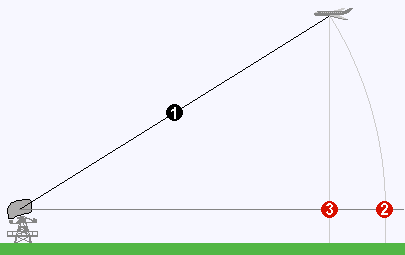
\includegraphics[scale=0.65]{./Figures/Slant_range.png}
\caption{Rango, altura y distancia a nivel de tierra. Imagen tomada de WolfgangW \citep{WolfgangW}. El rango inclinado (1) es la hipotenusa del triángulo representado por la altitud de la aeronave y la distancia entre la antena del radar y la trayectoria en tierra de la aeronave (punto (3) en la tierra directamente debajo de la aeronave). En ausencia de información de altitud, la ubicación de la aeronave se trazaría más lejos (2) de la antena que su trayectoria real en tierra.} 
\label{Rango_figura}
\end{figure}


El patrón de radiación de la antena se ilustra en la figura \ref{patrón_de_radiación} un haz estrecho cuando se ve desde arriba y, con cierta aproximación, puede considerarse como un trapecio si se ve de lado.


\begin{figure}
\centering
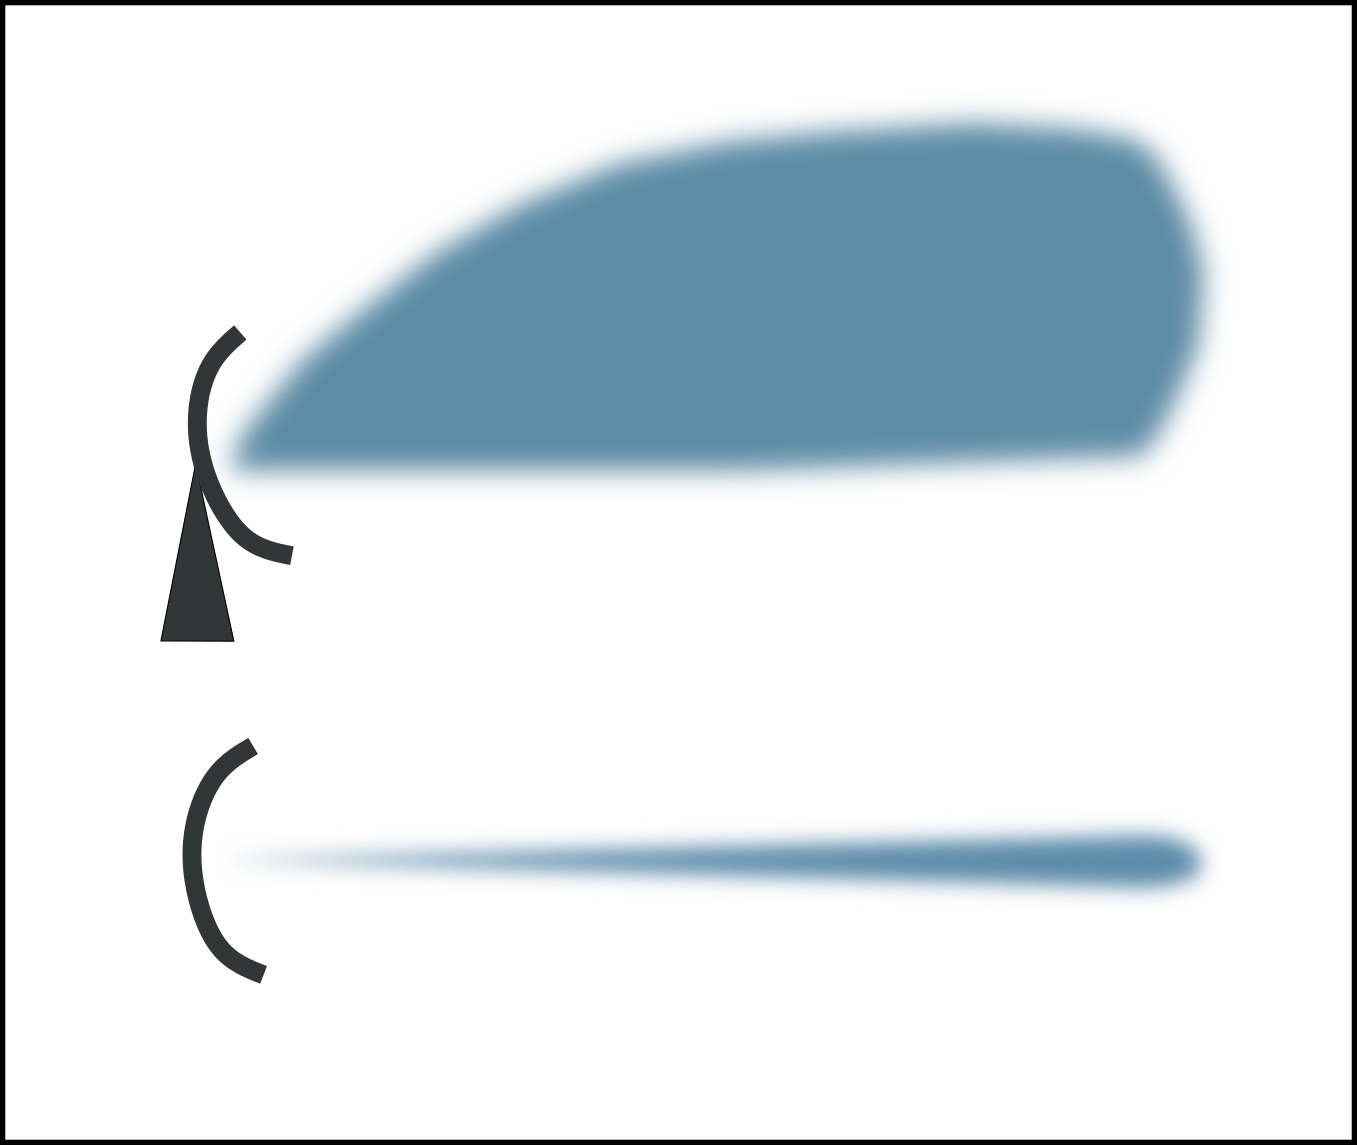
\includegraphics[scale=0.2]{./Figures/PSR_vistas.png}
\caption{Patrón de radiación de la antena.}
\label{patrón_de_radiación}
\end{figure}


Los radares que identifican objetos mediante la detección de reflexiones que estos producen de señales de radiofrecuencia se denominan radares primarios \citep{PSR}. Estos utilizan una antena que gira continuamente montada en una torre para transmitir ondas electromagnéticas que se reflejan, o se dispersan, desde la superficie de la aeronave hasta cierta cantidad de millas náuticas desde el radar. El sistema de radar mide el tiempo necesario para que el radar repita el eco y la dirección de la señal. A partir de esto, el sistema puede medir la distancia de la aeronave a la antena del radar y el azimut, o dirección, de la aeronave en relación con la antena.

Existen otro tipo de radares de vigilancia, denominados secundarios, que utilizan una segunda antena de baliza de radar unida a la parte superior de la antena del radar principal para transmitir y recibir datos del área de la aeronave para la altitud barométrica, el código de identificación y las condiciones de emergencia. Se emiten pulsos codificados, para realizar interrogaciones mediante trenes de pulsos. Las aeronaves militares, comerciales y algunas de aviación general tienen transpondedores que responden automáticamente a una señal del radar secundario informando un código de identificación y altitud. Los centros de control de tráfico aéreo utilizan estos datos del sistema para verificar la ubicación de la aeronave dentro de un radio determinado del sitio del radar. El radar secundario también proporciona una identificación rápida de aeronaves en peligro.

Se menciona a continuación algunas ventajas y desventajas de los radares primarios:
\begin{itemize}
\item
Ventajas
	\begin{itemize}
	\item
El radar primario es el único sensor de vigilancia utilizado en la aviación civil que no requiere ningún equipo a bordo para localizar la aeronave. A diferencia de radar secundario, puede descubrir una aeronave que experimente una falla de transpondedor o un intruso.
	\item
Se utiliza para captar objetivos de larga distancia. Puede detectar aviones desde una distancia de cientos de kilómetros.
	\item
Mantiene 360 grados de vigilancia desde la superficie hasta grandes altitudes. Determina la orientación de los objetivos en un área más grande.
	\end{itemize}

\item
Desventajas
	\begin{itemize}
	\item
	Cono de silencio. Debido al patrón de radiación, hay una parte del espacio aéreo sobre la antena que no se puede inspeccionar. Este efecto se mitiga colocando una serie de radares de tal manera que el cono de silencio de cada radar quede cubierto por otro radar.
	\item
	Los objetivos con el mismo rango de inclinación (en diferentes niveles) son difíciles de distinguir (las señales recibidas se superpondrán). Esto se mitiga combinando el radar primario con un radar secundario que puede reconocer las diferentes aeronaves por sus códigos de transpondedor.
	\item
	Límite de rango mínimo. El PSR opera en una frecuencia, lo que significa que no puede emitir y recibir señal al mismo tiempo. Si el objetivo está demasiado cerca de la antena del radar, la señal reflejada puede recibirse antes del final de la transmisión. Si eso sucede, el objetivo no será detectado. Tenga en cuenta que acortar el pulso también reducirá la cantidad de energía emitida, lo que limitará el alcance máximo del radar. Esto se mitiga ajustando la longitud del pulso y la velocidad de rotación de la antena.
	\end{itemize}
\end{itemize}


\subsection{Tipos de radares}
La tecnología de radar ha experimentado muchos cambios desde su invención. Actualmente existe diversa variedad de sistemas de radar \citep{RadarHandbook} que se pueden clasificar en varias categorías según la finalidad de uso, cantidad de antenas, dependencia del blanco (radares primarios y secundarios mencionados anteriormente), forma de onda, ámbito de aplicación, etc. A continuación se destacan algunos de los sistemas de radar más comunes:

\begin{itemize}
\item Radar biestático:
Consta de un transmisor y un receptor que están separados por una distancia que es igual a la distancia del objetivo esperado. Un radar en el que el transmisor y el receptor están ubicados en el mismo lugar se conoce como radar monoestático. La mayoría de los misiles tierra-aire y aire-aire de largo alcance emplean el uso de radar biestático.

\item Radar de onda continua:
En este tipo de sistema, la energía de una onda continua de radio, de frecuencia estable conocida, se transmite y luego se recibe de cualquiera de los objetos que reflejan las ondas. Un radar de onda continua utiliza tecnología Doppler, lo que significa que el radar será inmune a cualquier forma de interferencia de objetos grandes que estén estacionarios o se muevan lentamente.

\item Radar doppler:
Es una forma especial de radar que emplea el efecto Doppler para producir datos de velocidad sobre un objeto a una distancia determinada. Esto se logra enviando señales electromagnéticas hacia un objetivo y luego analizando cómo el movimiento del objeto ha afectado la frecuencia de la señal devuelta. Esta variación tiene la capacidad de proporcionar mediciones extremadamente precisas del componente radial de la velocidad de un objetivo en relación con el radar. Los radares Doppler tienen aplicaciones en diferentes industrias, incluida la aviación, la meteorología, la salud y muchas otras.

\item Radar monopulso:
Compara la señal recibida de un solo pulso de radar contra sí mismo con el objetivo de comparar la señal como se ve en múltiples polarizaciones o direcciones. La forma más común de radar monopulso es la adaptación de un radar de exploración cónico que compara el retorno de dos direcciones para medir directamente la ubicación del objetivo.

\item Radar pasivo:
Está diseñado para detectar y rastrear objetos procesando reflejos de fuentes de iluminación no cooperativas en el entorno. Estas fuentes incluyen por ejemplo señales de comunicaciones y transmisiones comerciales.

\item Radares de instrumentación:
Son radares que están diseñados para probar cohetes, misiles, aviones y municiones en campos de prueba gubernamentales y privados. Proporcionan una variedad de información que incluye espacio, posición y tiempo, tanto en tiempo real como en el análisis de post-procesamiento.

\item Radar meteorológico:
Este radar utiliza ondas de radio junto con polarización horizontal o circular. La selección de frecuencia del radar meteorológico depende de un compromiso de rendimiento entre el reflejo de la precipitación y la atenuación como resultado del vapor de agua atmosférico. Algunos radares meteorológicos están diseñados para utilizar cambios Doppler para medir la velocidad del viento y la polarización dual para identificar los tipos de precipitación.

\item Radares cartográficos:
Se utilizan para escanear una gran región geográfica en busca de aplicaciones geográficas y de teledetección. Están limitados a objetos relativamente estáticos. Existen algunos sistemas de radar específicos que pueden detectar a los humanos detrás de las paredes gracias a las características reflectantes de los humanos que son más diversas que las que se encuentran en los materiales de construcción.

\item Radares de navegación:
Poseen longitudes de onda cortas son capaces de reflejarse desde la tierra y las piedras. En su mayoría, son comunes en barcos comerciales y otros aviones comerciales de larga distancia. Hay varios radares de navegación que incluyen radares marinos comúnmente montados en barcos para evitar colisiones y con fines de navegación.

\end{itemize}


\subsection{Medición de distancia}
Tradicionalmente se ha considerado que estas ondas electromagnéticas se propagan en línea recta en el espacio y esto puede variar ligeramente según las condiciones atmosféricas y meteorológicas. Mediante el uso de antenas de radar especiales, esta energía se puede enfocar en la dirección deseada. De esta forma, se puede medir la dirección (en azimut y ángulo de ubicación ) de los objetos que reflejan.

El radar emite pulsos de radio cortos con una potencia de pulso muy alta. Este pulso se concentra solo en una cierta dirección de la antena y se propaga a la velocidad de la luz en esta dirección. Si hay un obstáculo en esta dirección, entonces parte de la energía del pulso se dispersa en todas las direcciones. Una parte muy pequeña también se refleja en el radar. La antena del radar recibe esta energía y un sistema electrónico evalúa la información contenida en esta señal de eco.

El rango está determinado por la diferencia de tiempo del pulso emitido y recibido (la velocidad de propagación es la velocidad de la luz) y la demora se obtiene del azimut de la antena. La velocidad de rotación de la antena suele estar entre 5 y 12 rpm. Como las distancias de viaje y retorno deben tenerse en cuenta en la medición, se utiliza la siguiente ecuación:

\begin{equation}
R = \dfrac{c_{0} t}{2}
\end{equation}

La distancia se suele indicar en "millas náuticas" (en inglés abreviado NM, Nautical Miles). El factor de conversión es \(1 NM = 1.852 km\).



\subsection{Interferencias}
El procesamiento de la señal de radar involucra filtrar distintos tipos de señales indeseadas que se superponen a la señal de eco recibida en el radar. La relación señal a ruido del sistema (Signal to Noise Ratio, SNR, por sus siglás en inglés) determina la capacidad del mismo para sobreponerse a la presencia de estas señales. Cuánto mayor sea la SNR del sistema, se puede aislar mejor los objetivos reales de las señales provenientes de fuentes de ruido del entorno. Las fuentes principales de estos ruidos se describen a continuación:

\begin{itemize}

\item
Ruido:
Es una fuente interna de interferencia que se origina en los componentes electrónicos. Como la potencia del eco recibido por el radar es muy baja, el receptor juega un papel clave en la minimización del ruido. La figura de ruido es una característica que permite	conocer el nivel de ruido producido por el receptor. Además de las fuentes internas, la radiación térmica natural del entorno constituye una fuente externa de interferencias, en particular la que rodea al blanco.

\item
Clutter:
Se denomina clutter a aquellos ecos recibidos por el radar que son, por definición, no deseados. Pueden estar causados por objetos del entorno, precipitaciones (lluvia, por ejemplo), tormentas de arena, animales (especialmente pájaros), turbulencias y otros efectos atmosféricos. 
\end{itemize}
	

\section{Procesamiento de la señal de radar}

La señal de vídeo analógico proveniente del radar por lo general viene con cierta cantidad de ruido y clutter incorporado. Los ecos de clutter son más intensos en zonas cercanas al radar y están influenciados por las condiciones atmosféricas. Se debe realizar un procesamiento sobre ésta señal de video para poder extraer la información sobre los blancos que circulen por el espacio aéreo cubierto por dicho radar. Se emplea para ello un procesador monoradar.

\subsection{Procesador monoradar}


El procesador monoradar tiene por misión la obtención de un dato, denominado plot, por cada blanco detectado por el radar. Es por ello que se encuentran ubicados en la cadena de proceso después de los procesos de filtrado  y detección. Normalmente los plots se proporcionan a través de un canal serie o sobre red en formato digital, donde cada blanco tiene asociados una serie de parámetros como la distancia, azimut, elevación (para radares tridimensionales), potencia, nivel de confianza, velocidad, etc. El procesador extrae estos parámetros a partir de las señales de vídeo proporcionadas por etapas previas. Utilizando estas señales, el procesador monoradar tiene que aglutinar la información procedente de un mismo blanco, debido a que el radar, de cada blanco, recibe un número de hits (reflejo de la emisión de un ciclo radar (PRF)) durante varios PRT consecutivos. El número de hits varía dependiendo del ancho del lóbulo de radiación, de la velocidad de giro de la antena, de la frecuencia de repetición de pulsos (PRF, Pulse repeticion frequency) del radar, del nivel de señal, de las condiciones meteorológicas, etc. Debido a esto el procesador monoradar, aplicando los algoritmos y procesos necesarios (ventana deslizante, por ejemplo), determinará los parámetros de azimut y distancia del blanco respecto a la estación Radar.


Por tanto, la función del procesador monoradar es, correlacionar toda la información procedente del blanco, agruparla y extraer la información útil (distancia, azimut, nivel de potencia, etc.), y proporcionar como salida la información correspondiente a un solo blanco, codificarlo en formato digital y enviarlo a consolas (locales o remotas) o a Centros de Fusión Remotos, donde se recibe este tipo de información de varios radares para presentar un solo blanco visto por varios radares de forma simultánea. De esta forma se pueden visualizar en centros de control remotos coberturas muy amplias.




\section{Técnicas CFAR}

Para limitar la cantidad de plots generados es necesario establecer un umbral de comparación a partir del cual se considera a un eco recibido como válido. Para limitar la cantidad de plots generados, no es suficiente establecer un umbral fijo de comparación para la señal recibida por el radar. Esto es debido a que la distribución de clutter en el espacio aéreo es variante con el tiempo y espacio, y con las condiciones atmosféricas. Por tanto la predicción de dicha distribución se vuelve difícil y es necesario emplear técnicas más avanzadas para mejorar la relación señal a ruido.

El presente trabajo adopta una solución basada en la técnica CFAR (acrónimo inglés de Constant False Alarm Rate), el cual emplea un umbral de comparación variable con el objetivo de tener una tasa de falsa alarma constante, que se adapta a las condiciones presentes en una determinada zona del espacio aéreo.


En general el sistema CFAR basa su funcionamiento en almacenar datos de vídeo en un cierto entorno para caracterizar una distribución de ruido en ese recinto (podemos considerar ruido al clutter y a otros tipos de interferencias). Esto luego es usado para evaluar si el eco recibido en ese entorno puede ser considerado como un blanco o no, dependiendo de la relación existente entre el ruido medio y la amplitud de tensión del eco. Como es de esperar, a mayor cantidad de datos de video almacenado, mejor caracterización del ruido. Para realizar esta función, el CFAR dispone de una celda bajo testeo, un cierto número de celdas, denomindas celdas de entrenamiento o de referencia, que almacenan el dato de amplitud del video digital en el entorno de la celda bajo testeo y una etapa que opera sobre estos datos para generar un umbral cuyo valor se comparará con la celda bajo testeo.

\subsection{CA-CFAR}

Existen diferentes técnicas CFAR. Empleando la técnica CFAR con promediado de celdas (CA-CFAR, por Cell-Averaging CFAR) se realiza un promediado de celdas llamadas celdas de referencia que se ubican a ambos lados de la celda bajo testeo. Es una técnica de aplicación general, ya que sirve para la mayoría de los casos. El ruido estimado se puede calcular como:

\begin{equation}
P_{n} = \dfrac{1}{N} \sum_{m=1}^{N} x_m
\end{equation}

donde \(N\) es la cantidad de celdas utilizadas y \(x_{m}\) es el valor de la muestra en cada celda. Si \(x_{m}\) resulta ser la salida de un detector de ley cuadrática, entonces \(P_{m}\) será la potencia de ruido estimada.




\begin{figure}
\centering
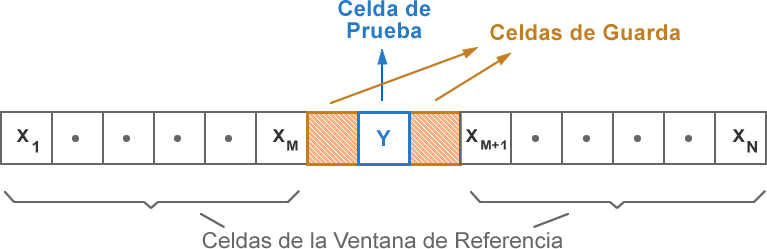
\includegraphics[scale=0.25]{./Figures/Estructura-del-Esquema-CA-CFAR.png}
\caption{Diagrama en bloques correspondiente al CA-CFAR.}
\label{fig:estructura_cfar}
\end{figure}

\subsection{Técnicas CA-CFAR relacionadas}

Para evitar introducir en la promediación la potencia proveniente de la celda bajo testeo, se establece alrededor de ella unas celdas de guarda, cuyo valor almacenado no se computa, sólo se transfiere a las celdas siguientes, como se ilustra en la figura \ref{fig:estructura_cfar}.

Existen variaciones inmediatas del algoritmo CA-CFAR \citep{CFAR_techniques}, en las cuales en lugar de considerar en la promediación de ruido los valores de ambas celdas de referencia, sólo se considera uno de ellos. Este es el caso de los algoritmos GOCA-CFAR (greatest of Cell-Averaging - CFAR) y SOCA-CFAR (smallest of Cell-Averaging - CFAR). Con estas técnicas se comparan los promedios parciales de las celdas de referencia y se considera el mayor o el menor respectivamente.

\subsection{Otras técnicas CFAR}
Existen otros algoritmos no considerados en este trabajo, que incorporan otras herramientas estadísticas, como ser OS-CFAR (por Ordered Statistic CFAR) y (TM-CFAR, por Trimmed Mean - CFAR):
\begin{itemize}
\item OS-CFAR
En la técnica CFAR de estadística ordenada, OS-CFAR, se ordenan las muestras de las celdas de referencia en orden ascendente. El elemento \(n/2\) es la mediana de los datos. El \(k-esimo\) elemento de la lista ordenada representa un determinado nivel de interferencia y el umbral es un múltiplo de este valor.
\item TM-CFAR
La técnica CFAR de constante media recortada (TM-CFAR), es una extensión de OS-CFAR en el que las celdas ordenadas en la ventana de referencia se recortan desde el extremo superior e inferior. El umbral es formado sumando las celdas restantes. En algunos TM-CFAR solo las celdas del extremo superior (celdas con mayor potencia) se descartan, por lo que si hay varios objetivos presentes en la ventana de referencia, el recorte elimina el efecto de la interferencia
objetivo.

\end{itemize}


\section{FPGA}

\begin{figure}
\centering
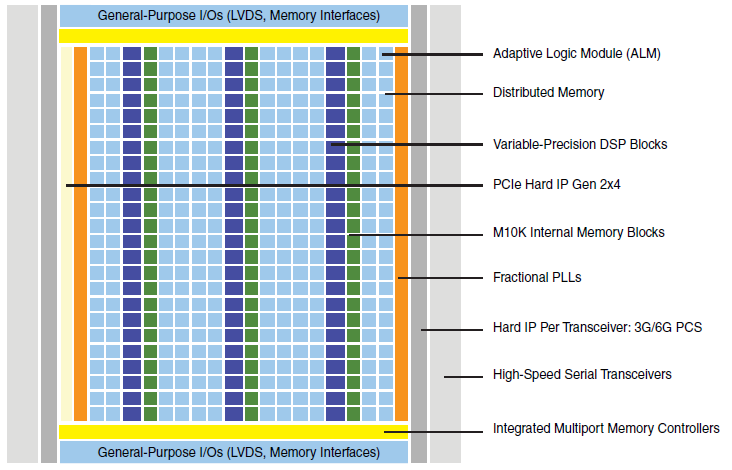
\includegraphics[scale=0.5]{./Figures/22-0.png}
\caption{Composición de una FPGA Cyclone V de Altera. Imagen tomada del Manual del chip.}
\label{fig:fpga_por_dentro}
\end{figure}

Las FPGA (por sus siglas en inglés, Field Programmable Gate Array) son una matriz de compuertas lógicas programables cuyos elementos se componen un conjunto de bloques lógicos configurables, conectados mediante conexiones programables \citep{FpgaArq}. Se crearon en el año 1984 como evolución de los dispositivos lógicos programables complejos (CPLD) y comparten ciertas similitudes con los Circuitos Integrados de Aplicación Específica, ASIC (acrónimo en inglés), sin embargo la diferencia con respecto a este viene marcada por su característica de ser reprogramable. También se pueden realizar comparaciones con otros dispositivos lógicos similares como GPP, DSP, ASIC estructurado, etc. Las FPGA se emplean en campos como la Medicina, procesamiento de imágenes y video, Aeroespacio y defensa, comunicaciones cableadas e inalámbricas, audio, entre otros \citep{fpga_xilinx}.

A diferencia con un microcontrolador, las FPGA no tiene una función específica incorporada, sino que poseen recursos para reproducir un circuito dentro del chip. Esto es posible debido los elementos lógicos individuales denominados CLBs (Configuble Logic Module) o  ALMs (Adaptative Logic Module), como se ilustra en la figura \ref{fig:fpga_por_dentro}. Las FPGA modernas incluyen en estos bloques elementos básicos como Flip Flops, Look-Up-Tables, Digital Signal Prossencing Blocks, relojes dedicados, PLLs, etc. Tambien tiene bloques de entrada y salida que se conectan con pines individuales de las ALMs, que pueden ejercer no sólo funciones de buffers sino también estados de alta impedancia.

Cabe mencionar que son dispositivos volátiles es decir que no tienen memoria, por sí solos no pueden almacenar su configuración de conexión y por tanto cuando se desconecta la fuente de energía se pierde esa configuración. Generalmente se utiliza una memoria por fuera de la FPGA para almacenar esa configuración.



\subsection{SoC-FPGA}

Los procesadores y las FPGA son dispositivos importantes en la mayoría de los sistemas embebidos. Los procesadores poseen la funcionalidad de gestión de alto nivel y las FPGA las estrictas operaciones en tiempo real, procesamiento de datos o funciones de interfaz.

Los dispositivos SoC-FPGA empezaron a producirse para brindar una alternativa de mayor desempeño y menor consumo y coste a sistemas que utilizan por separado una FPGA y un microprocesador o DSP. En los dispositivos SoC-FPGA se integra la arquitectura del procesador y FPGA en un sólo dispositivo. Esto brinda mayor integración, menor consumo de potencia, menor tamaño de placa y un mayor ancho de banda de comunicación entre el procesador y la FPGA \citep{soc_fpga}.

Como las señales entre el procesador y la FPGA ahora residen en el mismo chip, la comunicación entre los dos consume sustancialmente menos potencia en comparación con el uso de chips separados. Además la integración de miles de conexiones internas entre el procesador y la FPGA proporciona un ancho de banda mucho mayor y una latencia más baja que usar ambos dispositivos por separado.

El paso siguiente es incluir el chip dentro de una placa de circuito impreso (PCB, por el acrónimo inglés Printed Circuit Board). Para ellos hay empresas que ofrecen en el mercado PCB con diferentes tecnologías FPGA y variados periféricos. Un ejemplo es la placa tipo ADC-SoC, que incorpora una SoC-FPGA con un convertidor analógico a digital (ADC, por Analog to Digital Conveter) de alta velocidad.


\section{Bloques básicos de una FPGA}
En el presente trabajo se utilizó una FPGA de la firma Intel \citep{cycloneV_handbook}. A continuación se describe los componentes básicos que por generalmente incorpora una FPGA de esta empresa.

\subsection{ALM}

El bloque básico de una FPGA Cyclone V se denomina Adaptative Logic Module (ALM), el cual se ilustra en la figura \ref{ALM_diag_bloques}. Un ALM contiene cuatro registros programables, con los siguiente puertos:
\begin{itemize}
\item Data
\item Clock
\item Synchronous and asynchronous clear
\item Load
\end{itemize}

Las señales globales, los pines de entrada y salida de propósito general (GPIO)o cualquier señal interna de lógica pueden comandar las señales de control de clock y de clear de un registro ALM. Además los pines GPIO o la lógica interna controlan la señal de activación del reloj. Para las funciones combinacionales, los registros se omiten y la salida de la LUT es conducida directamente a las salidas de un ALM.

\begin{figure}
\centering
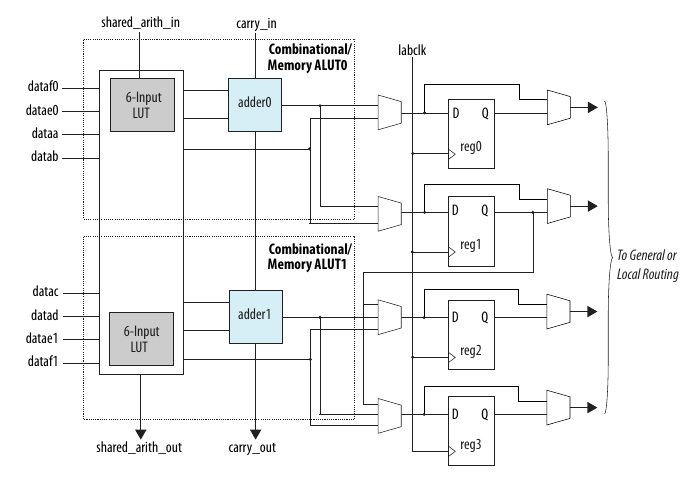
\includegraphics[scale=.75]{./Figures/diag_bloques_ALM.png}
\caption{Diagrama en bloques de un ALM. Imagen tomada del Manual del chip.}
\label{ALM_diag_bloques}
\end{figure}



\subsection{Bloques de memoria}

Posee además dos tipos de memorias embebidas, M10K y MLAB:

\begin{itemize}
\item
M10K: Las de tipo M10K son de 256 hasta 8000 bits de profundidad aproximadamente, están diseñadas para arrays extensos de memoria con puertos independientes.
\item
MLAB: Las de tipo MLAB sin embargo son de hasta 32 bits de profundidad y están optimizadas para la implementación de registros de desplazamientos, buffers tipo FIFO anchos y líneas de retardo. Cada MLAB se compone de diez ALMs y hasta el $25\%$ de las ALM se pueden configurar como memoria distribuida usando los bloques MLABs.
\end{itemize}

\subsection{Relojes y PLLs}
Posee 16 redes de reloj globales de 550 Mhz cuya arquitectura está basada en estructuras de Intel tipo globales, cuadrantes y periféricos. Esta estructura de reloj es compatible con pines de entrada de reloj dedicados y PLL fraccionales. Una característica importante del funcionamiento de los relojes es que en la herramienta Quartus identifica las secciones de la red de reloj sin usar y las desconecta, mejorando el consumo.


\subsection{Hard Processor System}
La FPGA posee integración con un sistema de procesamiento dentro del mismo chip. Este último se compone de una unidad de microprocesador con procesador córtex-A9 de ARM, controladores de memoria flash, soporte de periféricos y de interfaz, PLLs, interconexión SDRAM L3, entre otros.

Las partes HPS y FPGA del dispositivo SoC-FPGA son diferentes. El HPS arranca desde cualquiera de las múltiples fuentes de arranque, incluida la estructura FPGA y los dispositivos flash externos, y la FPGA se configura a través del HPS o cualquier fuente externa compatible con el dispositivo.





\section{Niveles de abstracción en el diseño digital}

En el ámbito del diseño digital se pueden distinguir diferentes niveles de abstracción \citep{niveles_abstraccion} que se distinguen por su impacto en el diseño y complejidad. Las decisiones a nivel conceptual son menos complejas pero tienen un impacto importante en el diseño final y a su vez la complejidad del diseño crece a medida que avanzamos en el ciclo del diseño. Podemos distinguir, por ejemplo, entre los siguientes niveles:

\begin{itemize}
\item
Nivel conceptual o de sistema:
Es el nivel más alto en el diseño. Consiste en captar los requerimientos y especificaciones del sistema y, a partir de los mismos, reducir opciones de diseño y algoritmos.

\item
Nivel algorítmico:
Consiste en implementar los algoritmos en lenguajes de alto nivel con la intención de determinar resultados sobre la viabilidad del diseño. Por ejemplo implementar una simulación usando lenguaje Python, lenguaje C/C++ o entorno MATLAB.
\item
Nivel de transferencia de registros:
En este nivel, también denominado RTL (por el acrónimo inglés, Register Transfer Level), se considera que el algoritmo ya está decidido y se procede a describir los detalles de cómo se mueven los datos entre y dentro de los subsistemas, además de cómo se manipulan los datos en función de las entradas del sistema. Su comportamiento se describe mediante un lenguaje de descripción de hardware (HDL, por el acrónimo de Hardware Description Language).
\item
Nivel de compuertas:
El código escrito en RTL se sintetiza para la implementación a nivel de compuerta. El proceso de síntesis toma el RTL y lo traduce, elaborando una lista de conexiones a nivel de puerta (netlist). Para la síntesis lógica, el usuario especifica restricciones de diseño y la tecnologı́a de destino en forma de una biblioteca de celdas estándar (cell library). La biblioteca tiene compuertas lógicas básicas estándar, como AND y OR, o macrocéldas como sumadores, multiplicadores, flip-flops, multiplexores, etc.
La herramienta convierte completamente el diseño descrito en RTL en un diseño que contiene celdas estándar. Para mapear de forma óptima la descripción de alto nivel en hardware real, la herramienta realiza varios pasos:
\begin{itemize}
\item
Convierte primero la descripción RTL en lógica booleana no optimizada.
\item
Realiza varias transformaciones para optimizar la lógica sujeto a restricciones de usuario, donde esta optimización es independiente de la tecnologı́a de destino.
\item
Finalmente, la herramienta mapea la lógica optimizada a celdas estándar específicas de la tecnología.
\end{itemize}


\item
Nivel de transistor
Es el nivel más bajo de abstracción, se describe el funcionamiento de las puertas y registros básicos utilizando transistores, cables y otros componentes eléctricos como resistencias y condensadores.

\end{itemize}



\section{Lenguaje de descripción de hardware}

Los lenguajes de descripción de hardware (HDL) se utilizan a nivel RTL para describir la estructura y comportamiento de sistemas digitales en forma textual. No son lenguajes de programación ya que a diferencia de estos, los HLDs pueden manejar múltiples procesos paralelos (como flip-flops y sumadores) que se ejecutan automáticamente de forma independiente entre sí. Cualquier cambio en la entrada del proceso activa automáticamente una actualización en la pila de procesos. En el proceso de diseño es importante tener en cuenta que cada línea de código representa uno o más componentes de hardware.
 
El uso de un lenguaje de descripción de hardware (HDL) para diseñar en dispositivos FPGA tiene las siguientes ventajas:
\begin{itemize}
\item
Enfoque de arriba hacia abajo (top-down) para proyectos grandes.
Este enfoque para el diseño de sistemas funciona bien para grandes proyectos que requieren que muchos diseñadores trabajen juntos. Una vez que el equipo de diseño determina el plan de diseño general, los diseñadores individuales pueden trabajar de forma independiente en secciones de código separadas.
\item
Simulación funcional al principio del flujo de diseño.
Probar la funcionalidad del diseño antes de que se implemente en el nivel RTL o en el nivel de puerta permite realizar los cambios necesarios desde el principio.

\item
Síntesis de código HDL para puertas. Sintetizando la descripción del hardware para apuntar a la implementación del dispositivo FPGA:

	\begin{itemize}
	\item
	Disminuye el tiempo de diseño al permitir una especificación de diseño de mayor nivel, en lugar de especificar el diseño a partir de los elementos base del dispositivo FPGA.
	\item
	Reduce los errores que pueden ocurrir durante una traducción manual de una descripción de hardware a un esquema de diseño.
	\item
	Permite que la herramienta de síntesis aplique técnicas de automatización (como los estilos de codificación y la inserción automática de entradas y salidas) durante la optimización del código original. Esto se traduce en una mayor optimización y eficiencia.
	\end{itemize}


\item
Permite probar diferentes implementaciones de diseño al principio del flujo de diseño. Utilizando la herramienta de síntesis para realizar la síntesis lógica y la optimización en puertas. Dado que el tiempo de síntesis es corto, se pueden explorar diferentes posibilidades arquitectónicas en el nivel de transferencia de registros (RTL).
\item
Reutilización del código de nivel de transferencia de registro (RTL).
Se puede reorientar el código de nivel de transferencia de registro (RTL) a nuevos dispositivos FPGA con mínimos cambios.
\item

\end{itemize}

Los lenguajes HDL soportados por la IEEE son Verilog-HDL y VHDL \citep{ieee_std} \citep{ieee_pkg}. VHDL es un lenguaje que inicialmente usaban los contratistas del Departamento de Defensa de EE.UU; ahora se usa comercialmente y en universidades de investigación. Verilog nació como un HDL exclusivo, promovido por una compañía llamada Cadence Data Systems, pero Cadence transfirió el control de Verilog a un consorcio de empresas y universidades llamado Open Verilog International (OVI). Actualmente OVI y Open VHDL Internacional se unieron para formar Accellera. Para este proyecto se empleó ambos lenguajes, los cuales se describirán a continuación.


\subsection{Aspectos básicos del lenguaje VHDL}
Un sistema digital está descrito por sus entradas y sus salidas y la relación que existe entre ellas \citep{intro_VHDL}. VHDL tiene una estructura que separa la declaración de puertos de entrada y de salida por un lado y por el otro la descripción del comportamiento del componente.
En la entidad (entity), se declaran los puertos de entrada y salida a utilizar, y en la sección arquitectura (architecture) se describe el comportamiento de la entidad, como se ilustra en la figura \ref{componente vhdl}. Cada arquitectura tiene asociada una entidad. Si es necesario, se pueden declarar bibliotecas a utilizar, por ejemplo para cálculo aritmético o para operación entre señales lógicas.

\subsubsection{Entidad de diseño}
La entidad de diseño es la principal abstracción en VHDL. Una entidad puede representar un sistema entero, un subsistema,una plaqueta, un chip, una macrocelda, una compuerta lógica o cualquier nivel de abstracción que se encuentre entre los antes mencionados.

Una entidad de diseño también puede describirse en términos de componentes interconectados. Cada componente de una entidad de diseño puede estar vinculada a una entidad de diseño de nivel inferior para definir la estructura o el comportamiento de ese componente, como se ilustra en la figura \ref{interconexión de componentes}. La separación de una entidad de diseño en componentes y la interconexión de esos componentes a otras entidades de diseño que pueden separarse de manera similar, da como resultado una jerarquía de entidades de diseño representando un diseño completo. Esta colección de entidades de diseño se denomina jerarquía de diseño. El bloque superior, denominado top-level, es un bloque externo y los bloques anidados en la jerarquía son bloques internos. El uso de jerarquías permite crear código reutilizable y crear componentes que realizan una función específica.

\begin{figure}
\centering
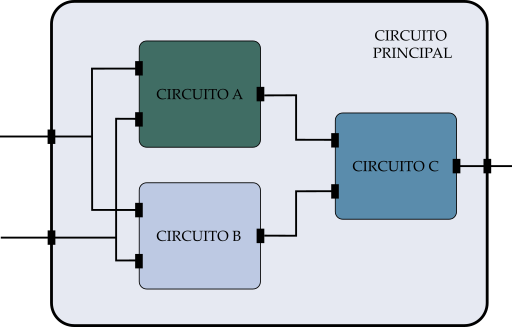
\includegraphics[scale=.5]{./Figures/vhdl_ejemplo2.png}
\caption{Circuitos A, B y C como instancias de un circuito principal.}
\label{interconexión de componentes}
\end{figure}


\subsubsection{Arquitectura de diseño}

La arquitectura define el cuerpo de una entidad de diseño. Especifica las relaciones entre las entradas y las salidas de esta, y puede estar expresada en términos de estructura, flujo de datos o comportamiento.


\begin{figure}
\centering
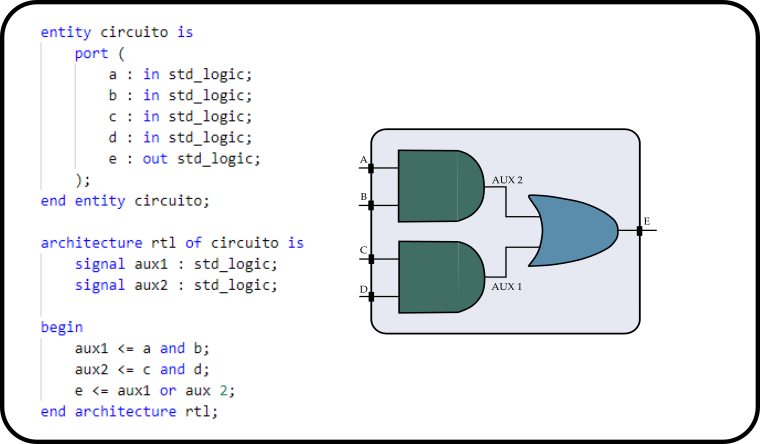
\includegraphics[scale=.65]{./Figures/vhdl_ejemplo.png}
\caption{Ejemplo de un componente descrito con VHDL.}
\label{componente vhdl}
\end{figure}

Dentro de la arquitectura se pueden crear las señales internas a esa entidad, que efectúan el proceso de las señales de entrada para proporcionar un cierto resultado en los puertos de salida. Para ello se utilizan procesos, asignaciones, instancias de componentes, registros y operaciones lógicas.

\begin{figure}
\centering
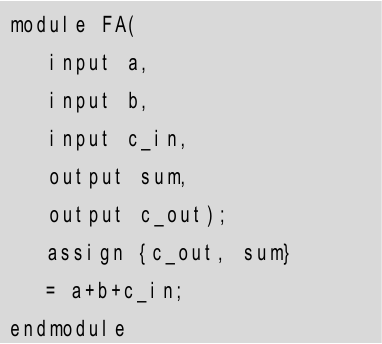
\includegraphics[scale=.95]{./Figures/verilog_ejemplo.png}
\caption{Ejemplo de un componente descrito con Verilog.}
\label{componente verilog}
\end{figure}

\subsection{Verilog}
Es un lenguaje de descripción de hardware que fue diseñado con una sintaxis similar a C. Puede operar a nivel RTL y de compuertas. El diseño se estructura mediante módulos,como se ilustra en la figura \ref{componente verilog}, que incluyen tanto declaración de puertos como el comportamiento.
Hay similitudes y diferencias en comparación con VHDL. Sin embargo, al parecer no hay una clara ventaja de usar uno u otro en términos de implementación.


\section{Flujo de diseno}
El diseño de un circuito digital involucra diferentes fases que se describen a continuación:

\subsection{Diseño}
Es la primer etapa del proceso. Consiste en ejecutar una toma de decisiones sobre el diseño a implementar y la manera de hacerlo. Esto implica tanto como determinar el tipo de placa, lenguaje HDL y herramientas a utilizar así como establecer jerarquías en el diseño y elaborar las especificaciones que deben cumplirse.


\subsection{Simulación}
Se utiliza una computadora para representar la estructura y comportamiento del sistema lógico digital \citep{morris_mano}. Mediante la simulación lógica, se interpreta la descripción HDL para predecir el comportamiento del hardware. De esta manera se pueden detectar errores en el funcionamiento del circuito antes de que se fabrique físicamente. Estos errores son corregidos modificando las sentencias del lenguaje empleado y sometiendo el diseño a un proceso de simulación. Una de las formas más usadas para simular diseños es el banco de pruebas (Testbench), que proporciona una forma gráfica de producir y visualizar las formas de onda de las señales de entrada y salida.



\begin{figure}
\centering

\includegraphics[scale=.5]{./Figures/test_bench3.png}
\caption{Diagrama en bloques de un test bench}
\label{diag test bench}
\end{figure}


El testbench no posee puertos de entrada ni de salida, sino señales de estimulación que se conectan a cada puerto de entrada del dispositivo bajo testeo o DUT (por el acrónimo inglés Device Under Test) y señales de observación que se conectar a los puertos de salida para observar la respuesta del DUT a esos estímulos, como se muestra en la figura \ref{diag test bench}.

Así, el proceso de simulación se resume en las siguientes etapas:

\begin{enumerate}
\item
Diseño del componente con HDL
\item
Diseño del marco de pruebas
\item
Verificación
\item
Corrección del componente
\end{enumerate}


\subsection{Síntesis}

En este proceso se emplea una herramienta de síntesis, proporcionada en general por el fabricante del chip, que elabora una lista de primitivas y sus interconexiones (netlist) a partir del diseño descrito en mediante HDL. La síntesis depende del dispositivo utilizado y de los recursos lógicos de los que disponga; diferentes dispositivos pueden implementar una misma función de distintas formas sin cambiar la funcionalidad del diseño. 

El grado de optimización del proceso de síntesis a la hora de convertir el código HDL al un circuito equivalente, depende de los siguientes factores:
\begin{enumerate}
\item La descripción del circuito.
Este punto es el más importante porque impacta en los recursos a utilizar y en las directivas a incluir. En la descripción además de decir qué función realiza el circuito, se describe la forma en la que debe realizarlo. Cuando se describe el funcionamiento de un circuito, existen muchas formas de hacer las mismas operaciones, y todas ellas darán lugar a distintas formas de implementación.

\item Los recursos disponibles en el dispositivo seleccionado.
Los recursos afectan a la forma en que las funciones descritas son interpretadas e implementadas en los bloques lógicos existentes en el dispositivo. Por ejemplo, un circuito que realice una división entre un número que no sea potencia de dos no podría hacerse en ciertos dispositivos, que no cuentan con esta característica.

\item Las directivas de síntesis seleccionadas por el diseñador.
Las directivas de síntesis son aquellos parámetros que se configuran para que la herramienta de síntesis los tenga en cuenta en el proceso de implementación. Por ejemplo, incluir restricciones de tiempo a ciertas señales permite que la implementación de los bloques que se conecten a dichas señales se realice de manera de ubicarlos en una sección del chip que permita que esta restricción se cumpla. En caso de que no se cumpla, la herramienta dará un error de síntesis para comunicar que el diseño debe ser modificado.
\end{enumerate}


\subsection{Implementación}
La implementación, también denominado como Place And Route (P \& R)en las FPGAs, consiste en situar el diseño sintetizado usando las celdas lógicas del dispositivo. La implementación transforma las Netlist de nivel medio creadas en la síntesis, y las mapea en la superficie de la FPGA, usando la lógica y los recursos internos disponibles. El archivo final es un Bitstream (.bit) que será el fichero final que se cargará en la FPGA.

\subsection{Configuración}
La configuración incluye la transferencia del fichero bitstream a la FPGA. Éste puede residir en una memoria no volátil como una PROM, o dentro de la FPGA (Muchas FPGA vienen con una memoria  interna capaz de mantener el fichero de configuración). El bitstream puede ser cargado en la FPGA mediante programación JTAG, a través de un procesador, microcontrolador u otro dispositivo externo.
\chapter{Materiales y métodos} % Main chapter title

\label{Chapter2}

%----------------------------------------------------------------------------------------
%	SECTION 1
% Aquí se mencionan los componentes que se utilizaron y la metodología empleada.
% Luego pueden ir las plaquetas que se diseñaron para el prototipo, esquemáticos,
% diagrama de flujo, dibujos en 3D, etc.
%----------------------------------------------------------------------------------------


El presente trabajo formó parte de un proyecto más grande. Consistió en la realización de dos sistemas, CFAR y configurador, los cuales eran subsistemas de un Procesador Monoradar.

La partición del diseño se realizó teniendo en cuenta las distintas funciones a realizar. Para este proyecto, el sistema CFAR se diseñó para generar el umbral adaptativo propio de la técnica mencionada. Luego, teniendo en cuenta que el clutter se concentra en general en las inmediaciones del radar y que se podría tener mejor desempeño en el filtrado admitiendo distintos factores de escala CFAR en distintas zonas de la cobertura, se diseño el sistema configurador para poder sectorizar la cobertura en un determinado número de sectores independientes. Además, se incorporó al configurador ciertas funciones para realizar un ajuste automático en el valor de escala CFAR para cumplir una determinada cantidad de presencia requerida por el usuario.

Para la realización del presente trabajo se utilizó:
\begin{itemize}
\item Placa ADC-SoC de TerasIC.
\item Software Quartus Prime.
\item Software ModelSim.
\item Software VHDL Style Guide.
\item Sistema de control de versiones GIT.
\item Repositorio remoto en GitHub.
\item Procesador monoradar preexistente.
\item Simulador de radar.

\end{itemize}

En las secciones siguientes se menciona la utilización de las mismas.

\section{Placa ADC-SoC de TerasIC}
Se utilizó una placa tipo SoC-FPGA de la firma TeraSiC. Esta placa posee un circuito de conversión analógica a digital que utiliza conectores SMA como interfaz de entrada y proporciona dos canales de conversión, cada uno de 14-bits de resolución y una frecuencia de muestreo de hasta 150 MSPS (Megasamples per Second).

\begin{figure}
\centering
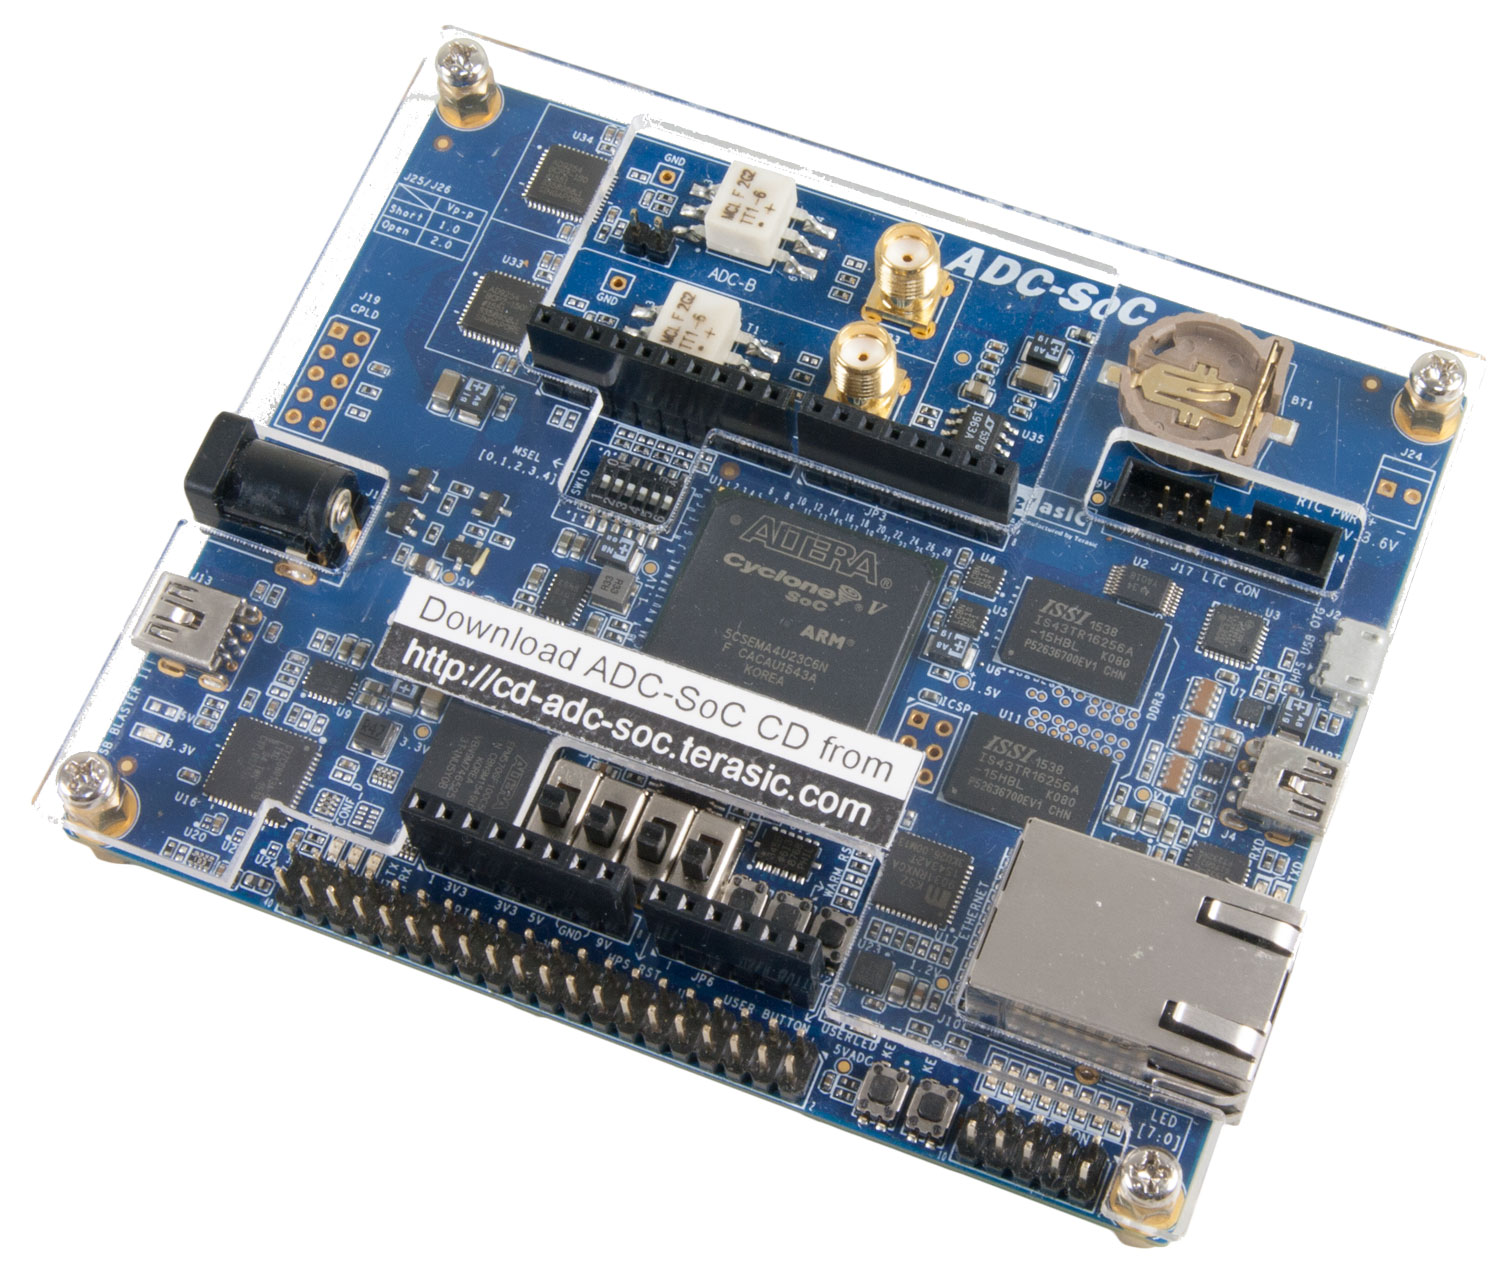
\includegraphics[scale=0.15]{./Figures/ADC-SoC.jpg}
\caption{Placa ADC-SoC de TerasIC}
\end{figure}

El siguiente hardware se proporciona en la placa:

\begin{itemize}
\item 	FPGA
	\begin{itemize}
	\item Dispositivo Altera Cyclone V.
	\item Dispositivo de configuración en serie.
	\item USB-Blaster II integrado para programación; Modo JTAG
	\item 2 pulsadores
	\item 4 interruptores deslizantes
	\item 8 LED de usuario verdes
	\item Tres fuentes de reloj de 50 MHz del generador de reloj
	\item Un cabezal de expansión de 40 pines
	\item Un encabezado de expansión Arduino (compatibilidad con Arduino Uno R3) donde se puede conectar los 'shields' Arduino.
	\item Un encabezado de expansión de entrada analógica de 10 pines (compartido con la entrada analógica Arduino).
	\item Convertidor A / D, interfaz SPI de 4 pines con FPGA
	\item  Dos convertidores AD de 14 bits con 150 MSPS (megamuestras por segundo)
	\end{itemize}
	
	
\item HPS (Hard Processor System)
	\begin{itemize}
	\item Procesador ARM Cortex-A9 de doble núcleo de 925 MHz
	\item 1GB DDR3 SDRAM (bus de datos de 32 bits)
	\item 1 Gigabit Ethernet PHY con conector RJ45
	\item Puerto USB OTG, conector USB Micro-AB
	\item Toma de tarjeta micro SD
	\item Acelerómetro (interfaz I2C + interrupción)
	\item UART a USB, conector USB Mini-B
	\item Botón de reinicio en caliente y botón de reinicio en frío
	\item Un botón de usuario y un LED de usuario
	\item Cabecera de expansión LTC 2x7
	\item RTC integrado (reloj en tiempo real)
	\end{itemize}
\end{itemize}


\begin{figure}
\centering
\includegraphics[scale=0.25]{./Figures/ADC-SoC_blockdiagram.jpg}
\caption{Diagrama en bloques de la placa ADC-SoC de TerasIC}
\end{figure}


En el chip Cyclone V de Altera (propiedad de Intel) se integra una FPGA y un HPS unidos por un puente HPS. Por defecto, la tarjeta micro SD tiene instalado el SO “​Linux Yocto Poky 8.0​”, el cual permite correr programas compilados en lenguaje C/C++ entre otros.
 
 
\section{Quartus Prime}
Como herramienta de compilación se utilizó \textit{Quartus Prime}, software producido por Altera para el análisis y la síntesis de diseños realizados en HDL. Permite compilar diseños, realizar análisis temporales, examinar diagramas RTL y configurar el dispositivo de destino con el programador.

\textit{Quartus} proporciona herramientas para trabajar en diferentes fases del diseño en FPGA como la creación del diseño, el agregado de restricciones, la compilación, el análisis de tiempos y la configuración de la FPGA con un programador. Se describen las características de \textit{Quartus} a continuación:

\begin{itemize}
\item
Creación del diseño: Es posible diseñar en nivel RTL con lenguajes VHDL, Verilog o SystemVerilog. Además posee una herramienta llamada \textit{Platform Designer} que crea automáticamente la lógica de interconexión a partir de la conectividad de alto nivel que se especifique. La automatización de interconexión elimina la laboriosa tarea de especificar conexiones HDL a nivel del sistema. De esta manera se pueden  especificar los requisitos de la interfaz e integrar componentes de IP dentro de una representación gráfica del sistema. En el presente proyectó se utilizó \textit{Platform Designer} (Diseñador de plataformas) para configurar el puente HPS.
\item
Permite el agregado de restricciones al diseño con herramientas denominadas \textit{assigment editor} (Editor de asignaciones) y \textit{pin planner} (Planificador de pines).
\item
Permite compilar el diseño, compuesto por las siguientes etapas:
\begin{itemize}
	\item
	Análisis y Síntesis
	Se evalúa el código para detectar la correcta escritura del mismo y se verifica que el mismo sea sintetizable, es decir que pueda ser implementado con lógica.
	\item
	\textit{Fitter} (Consiste en la colocación y Ruteo, \textit{Place \& Route}): Se asignan recursos específicos de la FPGA para cumplir con el diseño. En etapa etapa además la herramienta utiliza la información sobre las restricciones de tiempo evaluar qué celdas utilizar (en términos de propagación de señales). Por otro lado, luego de la colocación, se emplean técnicas de optimización en la asignación de recursos.
	\item
	Generación de archivos de programación: Se generan los archivos necesarios para programar la FPGA.
	\item
	 Análisis de tiempo: Verifica mediante la herramienta \textit{Timing Analyzer} que se cumplan con las restricciones de tiempo especificadas en el diseño. Por ejemplo los referidos a la generación de señales de reloj internas, derivadas de fuentes de señales de reloj externas.
	\end{itemize}
	
\item 
Posee una herramienta llamada \textit{Signal Tab Logic Analyzer} que permite realizar un debug mientras el sistema se ejecuta en la FPGA.

\end{itemize}

\subsubsection{Visores de netlist}
A medida que los diseños de FPGA crecen en tamaño y complejidad, la capacidad de analizar, depurar, optimizar y restringir el diseño es fundamental. \textit{Quartus} posee visores llamados \textit{RTL Viewer}, \textit{State Machine Viewer} y \textit{Technology Map Viewer} (visores de nivel de transferencia de registros, de máquina de estados y de mapa tecnológico, respectivamente). Cada uno permite ver representaciones esquemáticas de la estructura interna del diseño. Cada visor muestra una vista única del \textit{netlist} (lista de redes) que se producen en diferentes etapas de la compilación, como se ilustra en la figura \ref{fig:netlist_viewers}. Se describen a continuación:

\begin{figure}
\centering
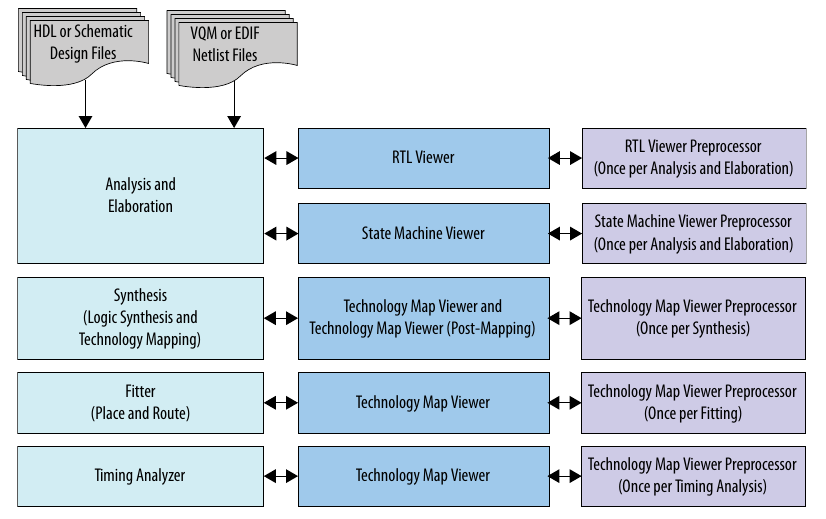
\includegraphics[scale=0.7]{./Figures/netlist_viewers.png}
\caption{Ubicación de los visores de netlist en el flujo de diseño de Quartus}
\label{fig:netlist_viewers}
\end{figure}

\begin{itemize}
\item
\textit{RTL Viewer}:
Permite ver un esquema de la lista de conexiones de diseño después de la etapa de Análisis y elaboración, y de la extracción de la lista de conexiones, pero antes de la síntesis y las optimizaciones de ajuste. Esta vista no es la estructura final del diseño, porque no se incluyen todas las optimizaciones; en cambio, es la vista más cercana posible al diseño original. Si el diseño utiliza síntesis integrada, esta vista muestra cómo \textit{Quartus} interpreta los archivos de diseño.

\item
\textit{State Machine Viewer}
Proporciona una vista de alto nivel de las máquinas de estados finitos en el diseño y muestra la estructura interna de las máquinas de estados en el diseño, incluida una vista más detallada de la entrada y salida de los nodos de estado individuales. También muestra las transiciones de los nodos en formato de tabla.

\item
\textit{Technology Map Viewer}
Permite ver un esquema de bajo nivel específico de la tecnología de la lista de redes de diseño después del ajuste o después de Análisis y síntesis. Se puede acceder a la vista del esquema \textit{post-fitting} (posterior al ajuste) o \textit{post-mapping} (posterior al mapeo), independientemente de la herramienta de síntesis que se utilice.

\end{itemize}


\subsection{ModelSim}

La simulación es un paso crítico en el diseño para FPGA. Permite al diseñador estimular su diseño y ver cómo el código que escribió reacciona al estímulo. Una gran simulación contendrá todos los estados posibles del diseño para garantizar que todos los escenarios de entrada se manejen de manera adecuada. Este ejercicio permite descubrir si en alguna parte del diseño, por ejemplo en procesos combinacionales,  no se contempló todos casos posibles y en caso de descubrir un comportamiento no esperado se procede a corregirlo.

Para este proyecto se utilizó ModelSim, un entorno de simulación creado por Mentor Graphics. ModelSim Está diseñado para trabajar con Verilog y VHDL. Además cuenta con un debugger, el cual se puede emplear, por ejemplo, para descubrir comportamientos más difíciles de dilucidar que no son determinados a simple vista.

\subsection{Buenas prácticas en la codificación VHDL}

\subsubsection{Guía de estilo de codificación VHDL}
Como se mencionó anteriormente, los sistemas desarrollados se diseñaron como subsistemas de un EDDR. Al ser el EDDR un proyecto más grande, involucró el trabajo de tres desarolladores y para unificar criterios de escritura del código VHDL se utilizó una guía de estilo de codificación.

Durante el proceso de revisión de código puede suceder que un problema real sea enmascarado por un problema de estilo de codificación. Dependiendo del proceso, los problemas de estilo pueden tardar mucho en resolverse. Por ejemplo, una serie de pasos a ejecutar podría ser:

\begin{itemize}
\item Crear una prueba.
\item Encontrar el problema.
\item Corregir el problema.
\item Verificar solución del problema.

\end{itemize}

Mantener un estilo de codificación permite por un lado, disminuir la probabilidad de errores y mejorar la lectura para uno mismo y para otros, especialmente durante el desarrollo del código en donde se comparte el trabajo con otros desarrolladores. Por el otro, dedicar menos tiempo a cuestiones de estilo deja más tiempo para analizar la estructura del código.

La eliminación de problemas de estilo reduce la cantidad de tiempo que se tarda en realizar las revisiones de código. Esto da como resultado una base de código de mayor calidad. Por ello, en este trabajó se utilizó un software, desarrollado por Jeremiah C Leary, denominado VSG (del acrónimo VHDL Style Guide).

Las características más destacadas de este programa son:
\begin{itemize}
\item
Definición explícita de los estándares de codificación VHDL.
\item
Configurable. Esto permite la actualización del código a los estándares actuales.
\item
Definición de un estilo del código y aplicación en partes o en toda la base del código.
\end{itemize}
El programa analiza el archivo cargado evaluando si el código cumple con todas las reglas de estilo, por ejemplo que todos los process tengan una etiqueta o que haya una correcta identación en las diferentes secciones del código. En caso de no hacerlo, VSG informará la regla que se viola y el número de línea o grupo de líneas donde ocurrió la violación. También da una sugerencia sobre cómo corregir la infracción.

La utilización de esta herramienta consistió en analizar cada entidad de diseño con el software y luego, realizar las correcciones pertinentes según el reporte de reglas incumplidas en cada archivo.

Para cuestiones que no están al alcance del software VSG se utilizó una convención para nombrar a puertos y señales

\subsubsection{Reglas de codificación}
Se adoptó las reglas de codificación propuestas por el departamento de sistemas informáticos de la Universidad Tecnológica de Tampere con el objetivo de aumentar la legibilidad para fines de revisión y evitar formas de codificación dañinas o poco prácticas. Se mencionan las más importantes a continuación:

\begin{itemize}
\item Usar solamente puertos tipo IN (de entrada) y tipo OUT (de salida).
\item Usar salidas registradas.
\item Realizar un \textit{test bench} por cada entidad de diseño.
\item Usar el flanco ascendente como flanco activo.
\item Hacer que los procesos síncronos sean sensibles sólo al \textit{clock} y \textit{reset}.
\item Hacer que los procesos combinacionales o asíncronos sean sensibles a todas las señales leídas en su interior.
\item Definir vectores en sentido descendente, tipo \textit{downto}.
\item Evitar números mágicos. Es decir, números que sólo el diseñador entiende de donde se originan. Emplear uso de constantes en su lugar.
\item Completar con todos los casos posibles las declaraciones secuenciales (por ejemplo \textit{if}, \textit{case}, etc).
\end{itemize}

\subsubsection{Otras convenciones}
Adicionalmente a lo mencionado anteriormente en ésta sección, se adoptaron convenciones propuestas por el equipo de desarrolladores del EDDR para nombres. Se mencionan a continuación:
\begin{itemize}
\item \textit{i\_ nombre} para puertos de entrada.

\item \textit{o\_ nombre} para puertos de salida.

\item \textit{nombre\_ s} para señales (cabe recordar que son de uso interno de la entidad).

\item \textit{nombre\_ v} para variables (función similar a señales).

\item \textit{i\_ nombre\_ numeración} para instancias.

\item \textit{nombre\_ g} para genéricos.

\end{itemize}


\section{Buenas prácticas en el diseño digital}

Al diseñar con código HDL, se debe comprender cómo una herramienta de síntesis interpreta las diferentes técnicas de diseño HDL y qué resultados esperar. Las diferentes técnicas de diseño pueden afectar la utilización de la lógica y el desempeño en cuanto al tiempo, así como la confiabilidad del diseño. Las buenas prácticas de diseño sincrónico están hechas para evitar la dependencia de los retrasos de propagación en un dispositivo, lo que puede provocar análisis de tiempos incompletos y posibles fallos. Se adoptó para este proyecto, las prácticas de diseño recomendadas por Altera (empresa fabricante del chip utilizado).


Se utilizó un diseño síncrono. En un diseño de este tipo, una señal de reloj controla la actividad de todas las entradas y salidas. El diseño se comporta de manera predecible y confiable para todas las condiciones de proceso, voltaje y temperatura (PVT) siempre que se asegure de que se cumplen todos los requisitos de temporización de los registros. Además es posible migrar fácilmente diseños síncronos a diferentes familias de dispositivos o grados de velocidad.


Se utilizó en todos los componentes los flancos activos del reloj parar disparar eventos. En cada flanco activo del reloj (que normalmente es el flanco ascendente), las entradas de datos de los registros se muestrean y se transfieren a las salidas. Siguiendo un flanco de reloj activo, las salidas de la lógica combinacional que alimentan las entradas de datos de los registros cambian de valor. Este cambio desencadena un período de inestabilidad debido a los retrasos de propagación a través de la lógica, ya que las señales pasan por varias transiciones y finalmente se establecen en nuevos valores. Los cambios que ocurren en las entradas de datos de los registros no afectan los valores de sus salidas hasta después del siguiente flanco de reloj activo. Debido a que el circuito interno de los registros aísla las salidas de datos de las entradas, la inestabilidad en la lógica combinacional no afecta el funcionamiento del diseño siempre que cumpla con los siguientes requisitos de tiempo:

\begin{itemize}
\item
Antes de un flanco de reloj activo, la entrada de datos haya sido estable durante al menos el tiempo de configuración del registro (\textit{setup time}).
  
\item
Después de un flanco de reloj activo, la entrada de datos permanezca estable durante al menos el tiempo de retención del registro (\textit{hold time}).
  
\end{itemize}

Al especificar todas las frecuencias de reloj y otros requisitos de tiempo, se puede utilizar la herramienta \textit{Timing Analyzer} descrita anteriormente para obtener un informe de los requisitos de hardware reales para los tiempos de configuración y tiempos de retención de cada pin del diseño. Al cumplir con estos requisitos de pines externos y seguir las técnicas de diseño sincrónico, se asegura el cumplimiento de los tiempos de configuración y retención para todos los registros del dispositivo utilizado.

Para cumplir con los requisitos de configuración y tiempo de espera en todos los pines de entrada, cualquier entrada a la lógica combinacional que alimenta un registro debe tener una relación sincrónica con el reloj del registro. Si las señales son asíncronas, se puede registrar las señales en las entradas del dispositivo para ayudar a prevenir una violación de los tiempos de retención y de configuración requeridos. Cuando no se cumplen estos requisitos, la salida de un registro puede oscilar la salida o establecer la salida en un nivel de voltaje intermedio entre los niveles alto y bajo llamado estado \textit{metaestable}. En este estado inestable, pequeñas perturbaciones, como el ruido en los rieles de alimentación, pueden hacer que el registro asuma el nivel de voltaje alto o bajo, dando como resultado un estado válido impredecible. Pueden producirse varios efectos indeseables, incluidos mayores retrasos de propagación y estados de salida incorrectos. En algunos casos, la salida puede incluso oscilar entre los dos estados válidos durante un período de tiempo relativamente largo.

\subsubsection{Lógica combinacional}

Las estructuras lógicas combinacionales constan de funciones lógicas que dependen únicamente del estado actual de las entradas. En las FPGA de Altera, estas funciones se implementan en LUT's con elementos lógicos o módulos lógicos adaptativos (ALM).

Los bucles combinacionales se encuentran entre las causas más comunes de inestabilidad y falta de fiabilidad en los diseños digitales. Los bucles combinacionales generalmente violan los principios de diseño síncrono al establecer un bucle de retroalimentación directa que no contiene registros. En un diseño síncrono, los circuitos de retroalimentación deben incluir registros. Por ejemplo, un bucle combinacional ocurre cuando el lado izquierdo de una expresión aritmética también aparece en el lado derecho en el código HDL. Un bucle combinacional también ocurre cuando retroalimenta la salida de un registro a un pin asincrónico del mismo registro a través de la lógica combinacional. En la sección siguiente se describirá una metodología que previene este tipo de bucles.

Otras recomendaciones tenidas en cuenta en el proceso de diseño fue la de evitar \textit{latches} inintencionales. Un \textit{latch} es un circuito pequeño con retroalimentación combinatoria que mantiene un valor hasta que se asigna un nuevo valor. Es común que los errores en el código HDL provoquen una inferencia de \textit{latch} no intencionada. A diferencia de otras tecnologías, un \textit{latch} en la arquitectura FPGA no es significativamente más pequeño que un registro. La arquitectura no está optimizada para la implementación de \textit{latches} y estos generalmente tienen un rendimiento de temporización más lento en comparación con los circuitos registrados equivalentes.



\subsection{Metodología estructurada}
\label{metodologia_estructurada}
Para algunos componentes se empleó la metodología propuesta por Jiri Gaisler de \textit{Gaisler Research}. Se realizó de esa manera para asegurar la síntesis en aquellos componentes donde había más procesamiento del tipo combinacional.

De acuerdo a autor, en el diseño  tradicional se presentan a menudo muchas declaraciones concurrentes, muchas señales y procesos de pocas líneas, entre otros. Esto puede ocasionar problemas, por ejemplo, en cuanto a:

\begin{itemize}
\item
Tiempo de ejecución (dependiendo del número de procesos).

\item 
Dificultad para entender el flujo de datos y/o el algoritmo.

\item
No distinguir entre señales del tipo secuencial y combinacional y señales relacionadas.

\end{itemize}

Para que el código sea fácil de entender y mantener, apto para rápida simulación, sintetizable y con menor posibilidad de discrepancias entre simulación y síntesis, el autor propone una abstracción de la lógica digital usando dos partes, como se ilustra en la figura \ref{2_process_scheme} , una secuencial y otra combinacional.

\begin{figure}
\centering
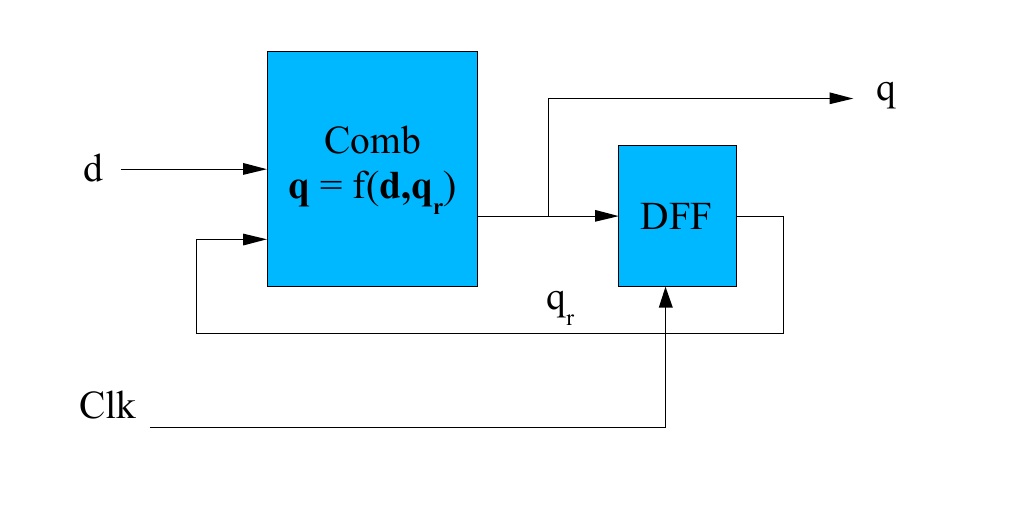
\includegraphics[scale=0.5]{./Figures/2_process_scheme.png}
\caption{Diseño sincrónico abstraído en dos partes, combinacional (izquierda) y secuencial (derecha)}
\label{2_process_scheme}
\end{figure}

Se implementó ésta metodología en VHDL de la siguiente manera:

\begin{itemize}
\item
La arquitectura albergó dos procesos: uno secuencial y otro combinacional.
\item
Se declaró dos señales locales, para entrada y salida del registro.
\item
Todo el algoritmo se volcó en el proceso combinacional.
\item
La lista de sensibilidad del proceso combinacional se realizó de modo que sea sensible a todos los puertos de entrada.
\item
La lista de sensibilidad del proceso secuencial se realizó de modo que sea sensible sólo a puerto de reloj.
\end{itemize}




\section{Diseño detallado}

\subsection{Requerimientos y especificaciones del proyecto}

Se detalla a continuación los requerimientos y especificaciones tanto para el CFAR como para el configurador:

\begin{itemize}
\item CFAR
	\begin{itemize}
	
	\item Requerimientos
		\begin{itemize}
		\item Diseñar un sistema CFAR que utilice los algoritmos CA-CFAR, GOCA-CFAR y SOCA-CFAR.
		\item Introducir automatismos al sistema CFAR para la variación del factor de escala que 			afecta al umbral de comparación.
		\item Implementar el diseño utilizando un HDL.
		\end{itemize}
	
	
	\item Especificaciones
		\begin{itemize}
		\item Emplear FPGA de la marca Intel.
		\item Emplear lenguaje de descripción de hardware VHDL.
		\item Realizar simulación de los componentes diseñados con simuladores de Quartus y 				ModelSim.
		\item Emplear sistema de control de versiones Git.
		\item Emplear repositorio remoto en GitHub.
		\end{itemize}

	\end{itemize}
\end{itemize}



\subsection{Partición Software $\&$ Hardware}
Uno de los primeros pasos para la realización de un diseño digital es la partición entre software y hardware. Es decir, decidir qué parte del diseñó se procesará con software y qué parte con hardware. A continuación se describe el detalle de la partición software/hardware para el CFAR y configurador:

\begin{itemize}
\item CFAR
	\begin{itemize}
	\item Componente de Firmware FPGA:
		\begin{itemize}
		\item Sistema CFAR de 32 celdas de referencia y 5 celdas de guarda.
		\item Posibilidad de alternar entre algoritmos CFAR.
		\item Celdas de 14-bit de resolución.
		\item Uso de coeficiente multiplicador de 16-bit.
		\end{itemize}
		
	\item Componente de Software HPS:
		\begin{itemize}
		\item Lectura de cuenta de targets (salida del CFAR).
		\end{itemize}
	
	\end{itemize}

\item Configurador
	\begin{itemize}
	\item Componente de Firmware FPGA:
		\begin{itemize}
		\item 64 sectores reducidos que abarquen cada uno una porción de la cobertura.
		\item 1 sector fijo que abarque toda la cobertura. 
		\item Posibilidad de alternar entre sector fijo y sectores reducidos.
		\item Control del tipo de video a utilizar (normal o integrado).
		\end{itemize}
	
	\item Componente de Software HPS:
		\begin{itemize}
		\item Control de coeficiente multiplicador.
		\item Control de coeficiente de ventana.
		\item Control del algoritmo.
		\item Control de tipo de filtrado.
		\item Control del modo de operación.
		\item Control del submodo de operación.
		\item Lectura de cuenta de multiplicador, algoritmo y ventana.
		\end{itemize}
		
	\end{itemize}
\end{itemize}

\subsection{Acciones del CFAR}
Se implementó la siguiente jerarquía de entidades de diseño para el CFAR:

\begin{itemize}
\item CFAR
	\begin{itemize}
	\item Celdas de referencia
		\begin{itemize}
		\item FFD
		\end{itemize}
	\item Celdas de guarda
		\begin{itemize}
		\item FFD
		\end{itemize}
	\item Celda test
	\item Comparador
	\end{itemize}

\item Contador CFAR

\end{itemize}

Cada componente fue diseñado para realizar las acciones que se describen a continuación.

\subsubsection{FFD}
\begin{itemize}
\item Debe funcionar como un registro de 14-bit de carga y salida paralela.
\item Debe transferir cada bit del vector en un flanco ascendente del reloj.
\item Debe resetearse de forma asincrónica.
\item Debe permitir habilitación o deshabilitación.
\end{itemize}



\subsubsection{Celdas de guarda}
\begin{itemize}
\item Debe comportarse como un registro de desplazamiento de 5 celdas.
\item Debe transferir el dato de video en cada flanco ascendente del reloj.
\item Debe resetearse de forma asincrónica.
\item Debe permitir habilitación o deshabilitación.
\end{itemize}


\subsubsection{Celdas de referencia}
\begin{itemize}
\item Debe comportarse como un registro de desplazamiento de 32 celdas.
\item Debe transferir el dato de video en cada flanco ascendente del reloj.
\item Debe resetearse de forma asincrónica.
\item Debe permitir habilitación o deshabilitación.
\item Debe proporcionar en cada flanco ascendente de reloj el cálculo de la suma todas del valor de video almacenado en todas las celdas.
\end{itemize}



\subsubsection{Celda Test}
Mismo comportamiento que FFD.

\subsubsection{Comparador}
\begin{itemize}
\item Debe recibir el valor de video digital almacenado en la celda bajo testeo.
\item Debe recibir la suma de las dos celdas de referencia.
\item Debe calcular la suma de las dos celdas de referencia.
\item Debe calcular el promedio de cada celda de referencia y el promedio total.
\item Debe recibir una señal de configuración para seleccionar uno de tres algoritmos posibles: CA-CGAR, GOCA-CFAR ó SOCA-CFAR.
\item Debe recibir un valor de multiplicador correspondiente a un factor de escala.
\item Debe generar un umbral con el multiplicador recibido y el promedio correspondiente al algoritmo seleccionado.
\item Además del umbral generado con el multiplicador recibido $x$, debe generar dos umbrales adicionales, uno con el multiplicador decrementado en una unidad $x-1$ y otro con el multiplicador incrementado en una unidad $x+1$.
\item Debe comparar el valor almacenado en la celda bajo testeo con cada umbral. Si el valor de la celda bajo testeo lo supera, deberá establecer cada salida correspondiente en un '1' lógico, de lo contrario deberá establecer cada salida correspondiente en un '0' lógico.
\end{itemize}


\subsubsection{CFAR}
\begin{itemize}
\item Debe recibir las señales de video digital proveniente de dos convertidores analógico a digital (ADC). Corresponde a los videos normal e integrado.
\item Debe permitir la selección de la fuente de video.
\item Debe contener dos celdas de referencia, dos celdas de guarda y una celda bajo testeo.
\item Debe permitir la selección de uno de tres algoritmos posibles: CA-CGAR, GOCA-CFAR ó SOCA-CFAR.
\item Debe obtener un umbral a partir de los multiplicadores(x, x+1 y x-1).
\item Debe proporcionar a su salida 3 señales de targets correspondiente a los umbrales (x, x+1 y x-1).
\end{itemize}



\subsubsection{Contador CFAR}
\begin{itemize}
\item Debe recibir los \textit{targets} (señal de salida del CFAR).
\item Debe utilizar la misma señal de reloj que el CFAR.
\item Debe incrementar una cuenta cada vez que se detecta un valor '1' lógico.
\item Debe proporcionar a la salida la cuenta en forma binaria.
\end{itemize}






\subsection{Acciones del configurador}
Se implementó la siguiente jerarquía de entidades de diseño para el configurador.

\begin{itemize}
\item Configurador
	\begin{itemize}
	\item Sector fijo
	\item Sector
		\begin{itemize}
		\item Registro de entrada
		\item Registro de salida
		\item Procesador de presencias
		\item Ajuste de multiplicador
		\end{itemize}

	\item Sectorizador
	\end{itemize}
\end{itemize}


Cada componente fue diseñado para realizar las acciones que se describen a continuación.

\subsubsection{Sector fijo}
\begin{itemize}
\item Debe almacenar la configuración existente en sus puertos de entrada cuando se detecte un flanco ascendente de reloj. La salida debe quedar disponible a partir de ese momento.
\end{itemize}

\subsubsection{Registro de entrada}
\begin{itemize}
\item Debe almacenar la configuración existente en sus puertos de entrada cuando se detecte un flanco ascendente de la señal de reloj y este coincida con un nivel alto de la señal correspondiente a la habilitación de carga de configuración. La salida debe quedar disponible a partir de ese momento.
\end{itemize}

\subsubsection{Registro de salida}
\begin{itemize}
\item Debe almacenar la configuración existente en sus puertos de entrada cuando se detecte un flanco ascendente de la señal de reloj y este coincida con un nivel alto de la señal correspondiente al paso por el norte del radar. La salida debe quedar disponible a partir de ese momento.
\end{itemize}

\subsubsection{Sector}
\begin{itemize}
\item Debe poder operar en dos submodos:
	\begin{itemize}
	\item Submodo fijo
	
	
		\begin{itemize}
		\item Debe operar únicamente con los registro de entrada y salida
		\item La carga de configuración en el registro de entrada estará habilitada sí y solo sí el código de sector que se encuentro dentro de la configuración sea igual al código de identificación de ese sector.
		\end{itemize}
	
	
	
	\item Submodo automático
		\begin{itemize}
		\item Debe contar las presencias
		\item En cada paso por el norte debe actualizar el multiplicador almacenado en el registro de salida en función de la cantidad de presencia requerida.
		\item En cada paso por el norte debe resetear los contadores.
		\end{itemize}
	
	
	\end{itemize}
\end{itemize}



\subsubsection{Procesador de presencias}
\begin{itemize}

\item Debe poder configurarse con el submodo en submodo fijo o automático.
\item En submodo fijo debe quedar inactivo con su salida en la decisión correspondiente a "no incrementar".
\item En submodo automático:
	\begin{itemize}
	\item Debe contar las presencias en tres contadores diferentes.
	\item Debe calcular el error absoluto de cada cuenta con la configuración de la cantidad de presencia requerida por el usuario.
	\item Debe decidir si para cada tipo de dato (correspondiente a cada contador) es necesario aumentar o disminuir el multiplicador para la siguiente vuelta.
	\end{itemize}

\end{itemize}

\subsubsection{Ajuste de multiplicador}
\begin{itemize}
\item Debe recibir el valor de decisión proveniente del procesador de presencias.
\item Debe contener una máquina de estados con dos estados, fijo y automático.
\item En modo automático debe modificar el valor del multiplicador almacenado de acuerdo a la decisión del procesador de presencias; puede aumentar o disminuir el valor del multiplicador o no modificarlo.
\item En modo fijo debe quedar inactivo proporcionando a la salida el último multiplicador modificado.
\end{itemize}

\subsubsection{Sectorizador}
\begin{itemize}
\item El grupo de puertos de entrada correspondientes a un sector determinado debe contemplar al menos los datos de selección de tipo de video, multiplicador, algoritmo y coeficiente de ventana.
\item Debe contener tantos grupos de entradas como salidas de configuración de los sectores se utilicen.
\item Debe generar el código de sector actual con las cuentas de rango y azimut.
\item Su salida debe funcionar como un multiplexor cuya llave de selección debe ser el código del sector actual.
\end{itemize}


\subsubsection{Configurador}
\begin{itemize}
\item Debe recibir las cuentas de rango y azimut de los subsistemas encargados de realizar esa cuenta.
\item Debe contar las presencias utilizando tres contadores diferentes.
\item Debe contemplar 2 modos de funcionamiento:
	\begin{itemize}
	\item Modo fijo (o manual): Debe proporcionar a la salida, un valor fijo de multiplicador, algoritmo, tipo de video y ventana deslizante para toda la cobertura.
	\item Modo automático: Debe generar el código de identificación de cada sector predefinido en base a la combinación de los datos de las cuentas de rango y azimut. Debe proporcionar a la salida la configuración almacenada en el sector correspondiente al sector por el que en ese intervalo de tiempo transita el radar.
	\end{itemize}
	
\item Los sectores instanciados deben ser independientes.
\item Debe recibir la configuración del puente HPS y redireccionar la misma al sector correspondiente si el modo de operación es automático o al sector fijo si el modo es fijo.
\item Su salida debe conectarse al CFAR para configurar su forma operación.
\item Debe contar con un multiplexor a la salida que, dependiendo del modo, direccione a los puertos de salida la configuración almacenada en el sector fijo o la que proviene del sectorizador.
\end{itemize}








	 
\chapter{Diseño e Implementación} % Main chapter title

\label{Chapter3} % Change X to a consecutive number; for referencing this chapter elsewhere, use \ref{ChapterX}
\definecolor{mygreen}{rgb}{0,0.6,0}
\definecolor{mygray}{rgb}{0.5,0.5,0.5}
\definecolor{mymauve}{rgb}{0.58,0,0.82}

\lstset{ %
  backgroundcolor=\color{white},   % choose the background color; you must add \usepackage{color} or \usepackage{xcolor}
  basicstyle=\footnotesize,        % the size of the fonts that are used for the code
  breakatwhitespace=false,         % sets if automatic breaks should only happen at whitespace
  breaklines=true,                 % sets automatic line breaking
  captionpos=b,                    % sets the caption-position to bottom
  commentstyle=\color{mygreen},    % comment style
  deletekeywords={...},            % if you want to delete keywords from the given language
  %escapeinside={\%*}{*)},          % if you want to add LaTeX within your code
  %extendedchars=true,              % lets you use non-ASCII characters; for 8-bits encodings only, does not work with UTF-8
  %frame=single,	                   % adds a frame around the code
  keepspaces=true,                 % keeps spaces in text, useful for keeping indentation of code (possibly needs columns=flexible)
  keywordstyle=\color{blue},       % keyword style
  language=[ANSI]C,					% the language of the code
  %otherkeywords={*,...},           % if you want to add more keywords to the set
  numbers=left,                    % where to put the line-numbers; possible values are (none, left, right)
  numbersep=5pt,                   % how far the line-numbers are from the code
  numberstyle=\tiny\color{mygray}, % the style that is used for the line-numbers
  rulecolor=\color{black},         % if not set, the frame-color may be changed on line-breaks within not-black text (e.g. comments (green here))
  showspaces=false,                % show spaces everywhere adding particular underscores; it overrides 'showstringspaces'
  showstringspaces=false,          % underline spaces within strings only
  showtabs=false,                  % show tabs within strings adding particular underscores
  stepnumber=1,                    % the step between two line-numbers. If it's 1, each line will be numbered
  stringstyle=\color{mymauve},     % string literal style
  tabsize=2,	                   % sets default tabsize to 2 spaces
  title=\lstname,                   % show the filename of files included with \lstinputlisting; also try caption instead of title
  morecomment=[s]{/*}{*/}%
}


%----------------------------------------------------------------------------------------
%	SECTION 1
%----------------------------------------------------------------------------------------








\section{Análisis del software}
 
La idea de esta sección es resaltar los problemas encontrados, los criterios utilizados y la justificación de las decisiones que se hayan tomado.

Se puede agregar código o pseudocódigo dentro de un entorno lstlisting con el siguiente código:

\begin{verbatim}
\begin{lstlisting}[caption= "un epígrafe descriptivo"]

	las líneas de código irían aquí...
	
\end{lstlisting}
\end{verbatim}

A modo de ejemplo:

\begin{lstlisting}[caption=Pseudocódigo del lazo principal de control.]  % Start your code-block

#define MAX_SENSOR_NUMBER 3
#define MAX_ALARM_NUMBER  6
#define MAX_ACTUATOR_NUMBER 6

uint32_t sensorValue[MAX_SENSOR_NUMBER];		
FunctionalState alarmControl[MAX_ALARM_NUMBER];	//ENABLE or DISABLE
state_t alarmState[MAX_ALARM_NUMBER];						//ON or OFF
state_t actuatorState[MAX_ACTUATOR_NUMBER];			//ON or OFF

void vControl() {

	initGlobalVariables();
	
	period = 500 ms;
		
	while(1) {

		ticks = xTaskGetTickCount();
		
		updateSensors();
		
		updateAlarms();
		
		controlActuators();
		
		vTaskDelayUntil(&ticks, period);
	}
}
\end{lstlisting}




% Chapter Template

\chapter{Resultados} % Main chapter title

\label{Chapter4} % Change X to a consecutive number; for referencing this chapter elsewhere, use \ref{ChapterX}

%----------------------------------------------------------------------------------------
%	SECTION 1
%----------------------------------------------------------------------------------------

\section{Resultados}
\label{sec: Resultados}

\subsection{Resultados del CFAR a ensayos con marcos de prueba}

\subsubsection{CFAR. Ensayo 1}
\label{Subsec:CFAR. Ensayo 1}

Se simuló el \textit{test bench} del CFAR para un intervalo de tiempo comprendido entre $0 us$ y $121 us$. La señal de estímulo del video de entrada se creó con las siguientes características para emular de manera aproximada una señal real:

\begin{itemize}
\item
Valor bajo equivalente al piso de ruido durante todo el periodo, excepto durante un pequeño intervalo de tiempo en la que adquiere un valor mayor. Se eligió como valor bajo \texttt{10000000000000} debido a que el conversor de alta velocidad es de 14-bit signado y el valor mencionado corresponde al cero. Físicamente el piso de ruido era cercano a cero. El valor de amplitud del pulso de video se eligió \texttt{10111011100000} como valor cercano al $50\%$ del rango de operación.


\item
Periódica de periodo suficientemente largo para que exista un solo pulso en el intervalo de tiempo que comprende la totalidad de celdas CFAR. La totalidad de las celdas CFAR generan un retardo indicado en la ecuación \ref{Eq:delay_cfar}, donde $N_{rc}$ es igual al número total de las celdas de referencia (128), $N_{gc}$ es igual al número total de las celdas de guarda (10) y $N_t$ es igual a el número total de las celdas bajo testeo (1).

\end{itemize}

\begin{equation}
T_{clk} *(N_{rc} + N_{gc} + N_t) =  0,8 us * 139 = 111,2 us
\label{Eq:delay_cfar}
\end{equation}



Se introdujo dos señales de reloj de diferentes periodos, de valores similares a los periodos reales. El primero para comandar la transferencia de datos entre las celdas CFAR y el segundo para realizar la comparación entre el umbral generado por el CFAR y el valor de video de la celda bajo testeo.

Se adoptó como valor inicial de multiplicador el valor $15784$ debido a que en ensayos preliminares con señal de radar real se observó que el mismo era un valor apropiado para determinar un rango útil de multiplicador.

En resumen, se introdujo los siguientes estímulos:
\begin{itemize}
\item Señal de reloj 1 de 800 ns de periodo.
\item Señal de reloj 2 de 20 ns de periodo.
\item Señal de algoritmo en "00". Correspondiente al algoritmo CA-CFAR.
\item Señal de video de entrada \texttt{video\_cf\_tb} de \texttt{14\-bit} tipo unsigned, periódica de periodo igual a 61 us, con valor \texttt{10000000000000} (8192 en sistema decimal) durante 60 us y \texttt{10111011100000} (12000 en sistema decimal) durante 1 us.
\item Señal de habilitación con valor permante en '1' lógico (siempre habilitado).
\item Señal de reset con valor permanente en '0' lógico (nunca resetea).
\item Señal de multiplicador inicializado en 15784 con incremento de una unidad en cada flanco ascendente del reloj 1.
\end{itemize}

El resultado de este ensayo se ilustra en la figura \ref{fig:cfar_ensayo_1}. Un acercamiento de la señal de multiplicador se ilustra en la figura \ref{fig:cfar_ensayo_1_zoom_multiplicador}.

\begin{figure}
\centering
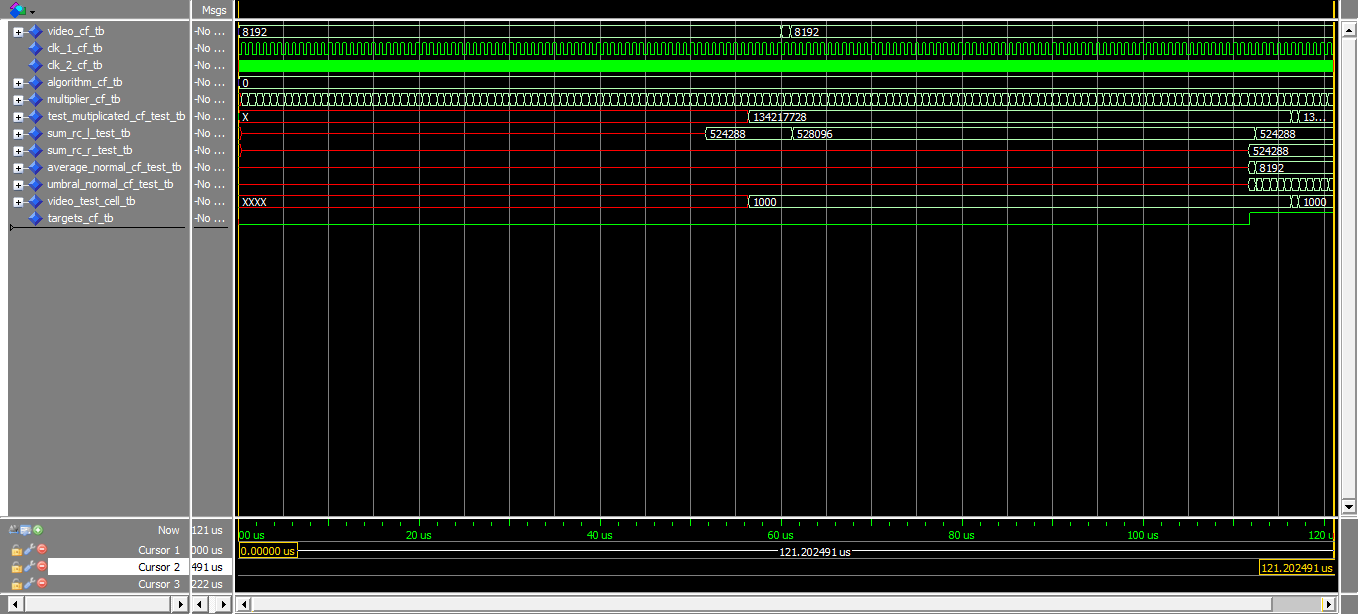
\includegraphics[scale=0.52, angle=270]{./Figures/cfar_ensayo_1.png}
\caption{CFAR. Ensayo 1 con \textit{testbench}}
\label{fig:cfar_ensayo_1}
\end{figure}

\begin{figure}
\centering
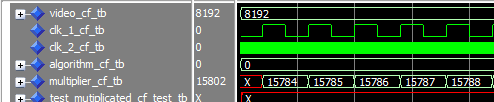
\includegraphics[scale=1]{./Figures/cfar_ensayo_1_zoom_multiplicador.png}
\caption{Acercamiento del ensayo 1. Variación del multiplicador}
\label{fig:cfar_ensayo_1_zoom_multiplicador}
\end{figure}



Se observó lo siguiente:

\begin{itemize}
\item
Las señales de estímulos se generaron adecuadamente.

\item
% (0.8*N)-0.4 = delay. N es el número de flanco.
Desde $0$ a $56,42 us$ la salida de la celda test estuvo indefinida. Esto se debe a la cantidad de flancos de reloj necesarios del reloj 1 para que el dato llegue a la celda  test, debiendo pasar antes por 64 celdas de referencia, 5 celdas de guarda y la propia celda test. Una vez que se actualizó la salida del la celda test se añade otro retraso interno al cfar, de un periodo del reloj 2, dado por el componente comparador, como se ilustra en la figura \ref{fig:cfar_ensayo_1_zoom_test_cell}. Este retraso debido al comparador se debe al tiempo que invierte el componente en realizar los cálculos de promediación y comparación para determinar si el video almacenado en la celda bajo testeo supera o no el umbral, la actualización de los datos de entrada y salida de este componente son dados en los flancos descendentes del reloj 2 para crear un desfase de $180º$ respecto del reloj 1 y asegurar la estabilidad del dato. Por último, se suma un retardo adicional de un periodo del reloj 1, correspondiente al registro de salida del cfar.

\begin{figure}
\centering
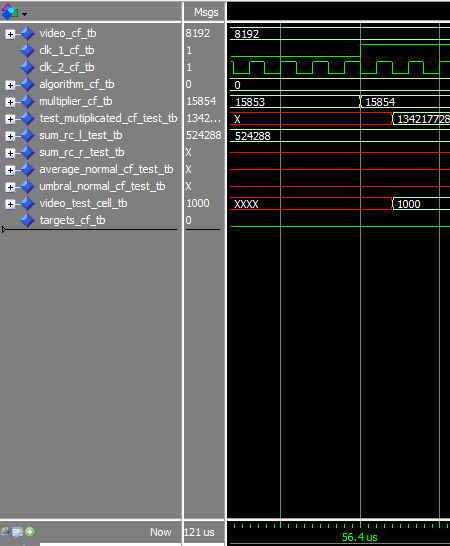
\includegraphics[scale=1]{./Figures/cfar_ensayo_1_zoom_test_cell.png}
\caption{CFAR.Ensayo 1. Acercamiento al tiempo $t=56.4 us$}
\label{fig:cfar_ensayo_1_zoom_test_cell}
\end{figure}


\item
Las señales de salida \textit{test\_mutiplicated\_cf\_test\_tb} y \textit{o\_test\_mutiplicated\_cfar}, actualizaron sus valores simultáneamente. El primero corresponde a la salida de la celda test; se actualizó al valor \texttt{134217728}, correspondiente a una corrección dada por la ecuación \ref{Eq:corrección_test_cell}, donde: $V_{tc corregido}$ es la corrección sobre el valor de video almacenado en la celda test, $V_{tc}$ es el valor de video almacenado en la celda test y $2^{14}$ es la resolución del ADC de alta velocidad. La segunda señal corresponde al puerto de salida del cfar de la celda test; se actualizó al valor \texttt{1000} (en sistema binario) debido a que representa en el sistema binario a una porción del valor de la celda test. Ocurre algo similar luego de $60 us$ cuando llega el pulso de video a la celda test.

\begin{equation}
V_{tc   corregido} = V_{tc} * 2^{14} = 8192 * 16384 = 134217728
\label{Eq:corrección_test_cell}
\end{equation}

\item
Desde 0 a 51,61 us la salida de la suma de todas las celdas de referencias ubicadas a la izquierda de la celda test, \texttt{sum\_rc\_l\_test\_tb}, se encuentra indefinida. Este retraso se ilustra en la figura \ref{fig:cfar_ensayo_1_zoom_sum_rc} y, como se indica en la ecuación \ref{Eq:delay_suma_rc_l}, se debe a la cantidad de flancos de reloj 1 necesarios para que el dato pase por todas las celdas y sea posible realizar la suma de sus valores almacenados, más un retraso adicional de 1 periodo del reloj 2, debido al registro de salida incorporado dentro del cfar. Luego de ese intervalo de tiempo la suma se actualizó al valor $8192 * 64 = 524288$, debido a que todas las celdas de referencia ubicadas a la izquierda de la celda test almacenaron el valor constante de $8192$. Se puede realizar un análisis similar para la celda de referencia ubicada a la derecha de la celda test, que dejó de estar indefinida a los $111,6 us$ debido al tiempo necesario para superar el retardo generado por sus celdas de referencia y las celdas anteriores, como se indica en la ecuación \ref{Eq:delay_suma_rc_r}.

\begin{figure}
\centering
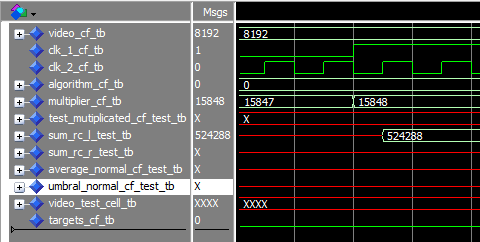
\includegraphics[scale=1]{./Figures/cfar_ensayo_1_zoom_sum_rc.png}
\caption{Acercamiento del ensayo 1. Detalle de la suma de salida de la celda de referencia izquierda}
\label{fig:cfar_ensayo_1_zoom_sum_rc}
\end{figure}

\begin{equation}
T_{clk 1} * N_{rc} - \dfrac{T_clk_1}{2} + \dfrac{T_clk_2}{2} = 0,8 us * 64 - 0,4 us + 0,02 us= 56,4 us
\label{Eq:delay_suma_rc_l}
\end{equation}


\begin{equation}
0,8 us *(64 + 64 + 5 + 5 + 1) + 0,4 us = 111,6 us
\label{Eq:delay_suma_rc_r}
\end{equation}

\item
A los 111,62 us, medio periodo del reloj 2 luego de haber quedado definido la sumas de la celda de referencia izquierda y, por tanto, teniendo disponible la suma de ambas celdas de referencia, se crea el promedio normal, como se ilustra en la figura \ref{fig:cfar_ensayo_1_zoom_umbral}. El promedio normal está compuesto por la suma de ambas celdas de referencia dividido 128, valor correspondiente a la cantidad total de celdas de ambas celdas de referencia. También en la figura\ref{fig:cfar_ensayo_1_zoom_umbral} se observó que $60 ns$ después de que el promedio normal (retraso necesario para efectuar el cálculo), la señal de salida del umbral normal adquirió un valor definido. El mismo adquierió el último valor de la multiplicación del promedio por el multiplicador, como se indica en la ecuación \ref{Eq:Ecuación del umbral normal}. A partir de ese momento, su valor creció en cada flanco ascendente del reloj 1 debido a que se encuentra afectado por el multiplicador.

\begin{figure}
\centering
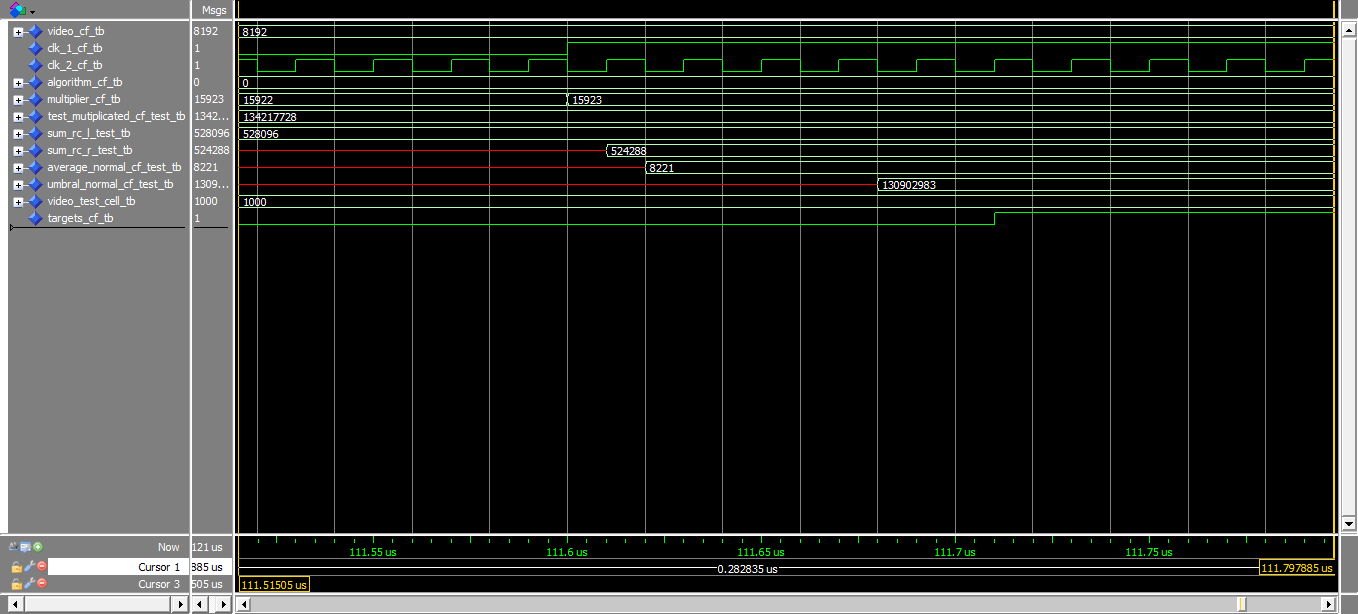
\includegraphics[scale=0.52, angle=270]{./Figures/cfar_ensayo_1_zoom_umbral.png}
\caption{CFAR. Ensayo 1 con \textit{testbench}, zoom alrededor de los 111,65 us}
\label{fig:cfar_ensayo_1_zoom_umbral}
\end{figure}

\begin{equation}
umbral_{normal} = promedio_{normal} * multiplicador = 8221 * 15923 = 130902983
\label{Eq:Ecuación del umbral normal}
\end{equation}

\item
Se observó a partir de los $111,68 us$ y hasta el final de la simulación ($121 us$), el nivel alto del puerto de salida del cfar correspondiente al target. Un nivel alto en un determinado instante de tiempo indica que en ese momento el valor de video almacenado en la celda test superó al umbral generado. Por tanto supondría un posible blanco.

\end{itemize}



\subsubsection{CFAR. Ensayo 2}
\label{Subsec:CFAR. Ensayo 2}

Se simuló el \textit{test bench} del CFAR para un intervalo de tiempo comprendido entre $121 us$ y $242 us$. Las señales estímulo utilizadas son las mismas que fueron descritas en las sección \ref{Subsec:CFAR. Ensayo 1}. Se ilustra el resultado de la simulación en esta porción de tiempo en la figura \ref{fig:cfar_ensayo_2}.

\begin{figure}
\centering
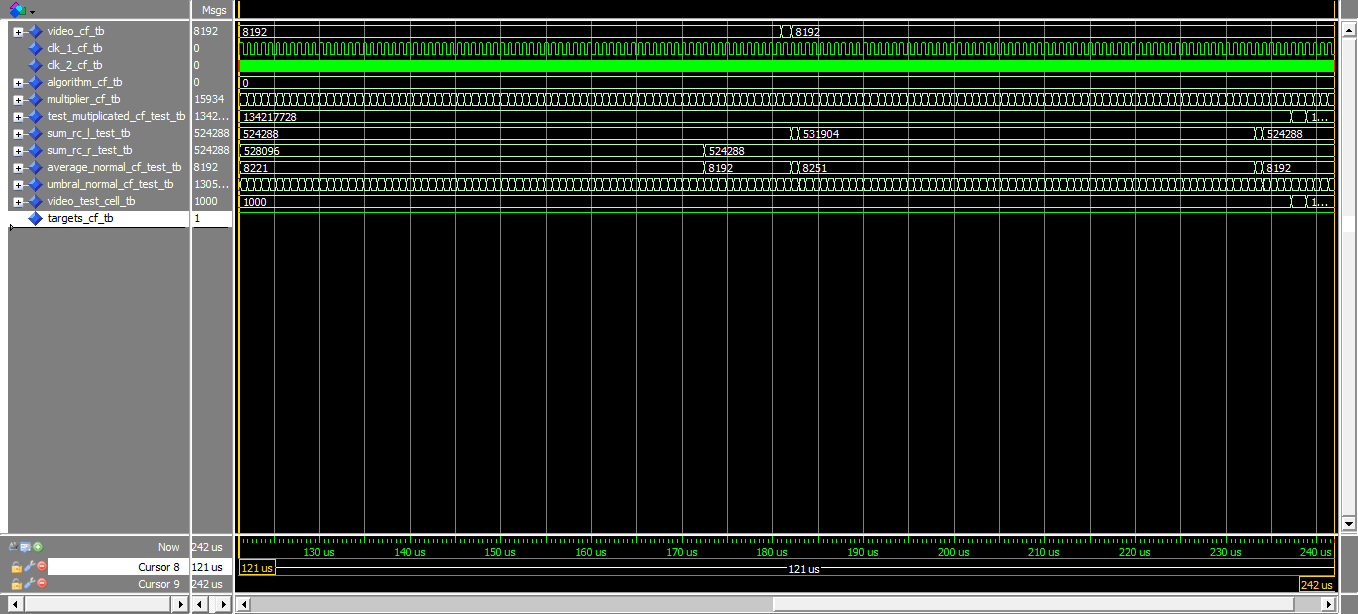
\includegraphics[scale=0.52, angle=270]{./Figures/cfar_ensayo_2.png}
\caption{CFAR. Ensayo 2}
\label{fig:cfar_ensayo_2}
\end{figure}


Se observó resultados similares a los descritos en la sección \ref{Subsec:CFAR. Ensayo 1}. Con diferencias en lo siguiente:

\begin{itemize}
\item
Valores definidas para todas las salidas.

\item
Valor del puerto de salida en nivel alto (1 lógico) durante todo el intervalo de tiempo de ensayo. Esto se debió a que el multiplicador se incrementa linealmente, una unidad en cada flanco ascendente del reloj 1 y hasta el final de la simulación, no adquiere el valor necesario para desplazar el umbral normal por encima del valor máximo del video de entrada.
\end{itemize}



\subsubsection{CFAR. Ensayo 3}
\label{Subsec:CFAR. Ensayo 3}

Se introdujo las señales de estímulo mencionadas en la sección \ref{Subsec:CFAR. Ensayo 1} con diferencia en la señal de video al cfar, compuesta de la siguiente manera:

\begin{itemize}
\item Señal de video de entrada \texttt{video\_cf\_tb} de \texttt{14\-bit} tipo unsigned, periódica de periodo igual a 500 us, con valor \texttt{10000000000000} (8192 en sistema decimal) durante 249.5 us, \texttt{10111011100000} (12000 en sistema decimal) durante 1 us y \texttt{10000000000000} durante 249.5 us.
\end{itemize}

Se simuló el \textit{testbench} del CFAR desde 0 us a 500 us para observar el comportamiento de las sumas de las celdas de referencia, el promedio normal y el umbral normal ante un sólo pulso en un rango de tiempo amplio. El resultado se ilustra en la figura \ref{fig:cfar_ensayo_3}.

\begin{figure}
\centering
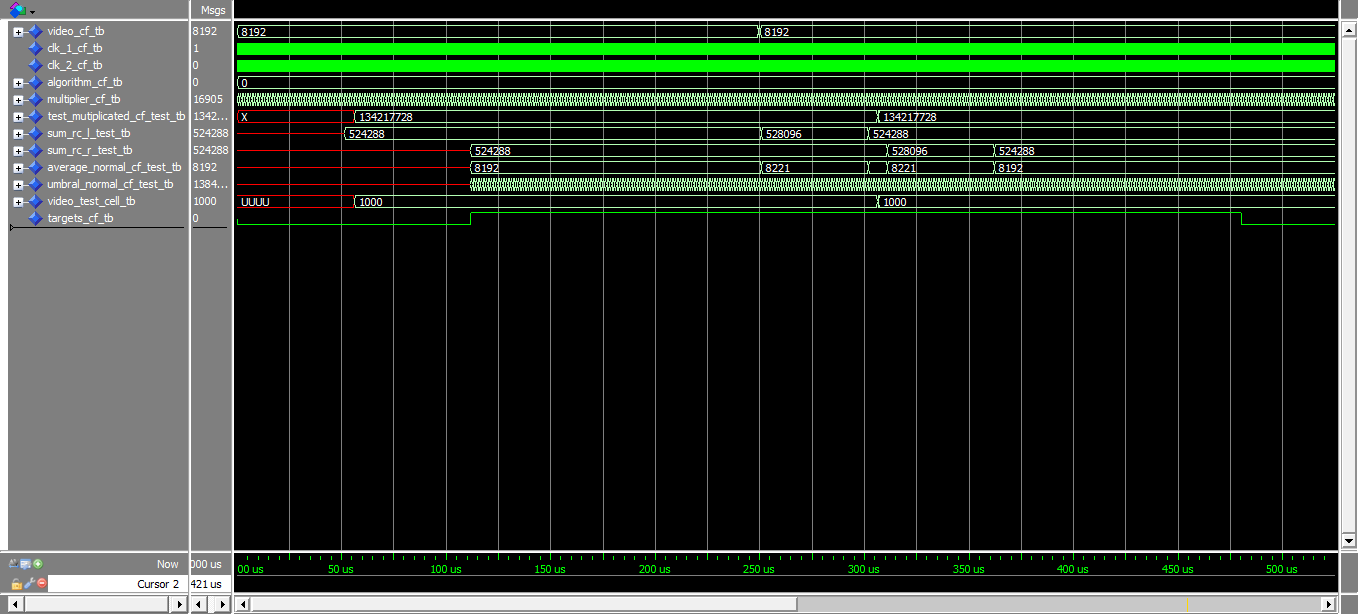
\includegraphics[scale=0.52, angle=270]{./Figures/cfar_ensayo_3.png}
\caption{CFAR.Ensayo 3}
\label{fig:cfar_ensayo_3}
\end{figure}

Se observó una variación escalonada en las señales de salidas correspondiente a ambas sumas de las celdas de referencia y en el promedio normal. Esto fue causado por el recorrido del pulso entre las celdas del CFAR. Se observó que antes y después del paso del pulso, las sumas y el promedio normal se mantienen estables en el valor \texttt{10000000000000} (8192 en sistema decimal). La variación de las sumas se ilustra en la figura \ref{fig:sumas_celdas}. La celda de referencia ubicada a la derecha de la celda test(azul), luego de 60 us, adquiere los mismos valores que la celda de referencia ubicada a la izquierda (rojo).

\begin{figure}
\centering
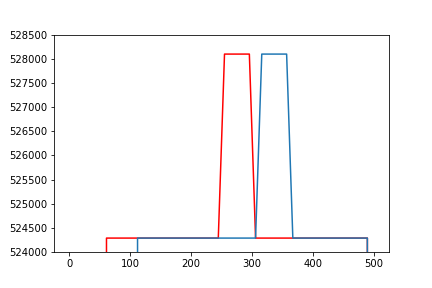
\includegraphics[scale=0.5]{./Figures/cfar_ensayo_3_sumas.png}
\caption{Variación de sumas de celdas de referencia.}
\label{fig:sumas_celdas}
\end{figure}



\subsubsection{CFAR. Ensayo 4}
\label{Subsec:CFAR. Ensayo 4}

Esta simulación comprendió el intervalo de tiempo entre $0 us$ y $7000 us$. El objetivo fue observar la comportamiento de la señal de salida del CFAR correspondiente al target. El resultado se ilustra en la figura \ref{fig:cfar_ensayo_4}.

Se observó que a los $480,47 us$ el multiplicador alcanza el valor $16384$. A partir de ese momento el valor de video almacenado en la celda test superó al umbral sólo en los momentos en donde su valor correspondió al pulso de valor \texttt{10111011100000} (12000 en sistema decimal). Durante toda la simulación el valor del multiplicador se incrementó linealmente, al igual que el umbral normal.

El nivel alto del puerto de salida del CFAR, correspondiente al target, se observó con un comportamiento periódico de acuerdo a lo mencionado en el párrafo anterior. A los $6806.02 us$ la celda test presentó un valor correspondiente al pulso de video, pero no se observó nivel alto del puerto de target debido a que en ese momento el multiplicador alcanzó un valor que incrementó el umbral a un nivel superior al valor máximo del CFAR. Este valor fue $24291$. Teniendo en cuenta la expresión de la ecuación \ref{Eq:Ecuación del umbral normal} y la correción del valor almacenado en la celda bajo testeo, indicada en la ecuación \ref{Eq:corrección_test_cell}, se verificó los datos arrojados en la simulación. Estos valores se ilustran en la figura \ref{fig:cfar_ensayo_4_zoom}, la cual es una imagen ampliada de la figura \ref{fig:cfar_ensayo_4}.

\begin{figure}
\centering
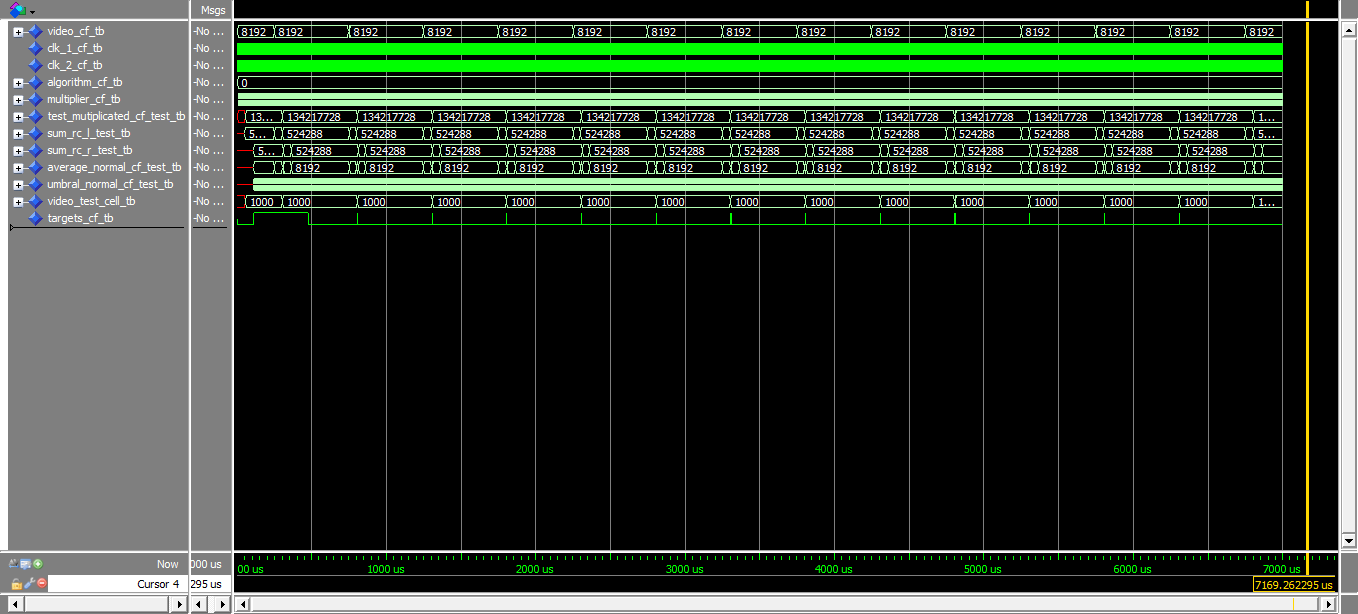
\includegraphics[scale=0.52, angle=270]{./Figures/cfar_ensayo_4.png}
\caption{CFAR.Ensayo 4}
\label{fig:cfar_ensayo_4}
\end{figure}
	
\begin{figure}
\centering
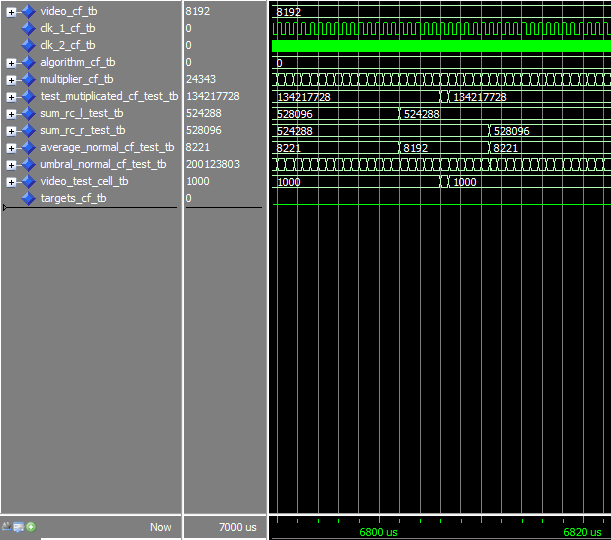
\includegraphics[scale=0.7, angle=0]{./Figures/cfar_ensayo_4_zoom_multiplicador.png}
\caption{CFAR.Ensayo 4. Acercamiento al tiempo $t=6806.02 us$}
\label{fig:cfar_ensayo_4_zoom}
\end{figure}

\subsection{Resultados del Configurador a ensayos con marcos de prueba}


\subsubsection{Configurador. Ensayo 1}
\label{Subsec:Configurador. Ensayo 1}

Se simuló el \textit{test bench} del componente \textit{sectorizador}, instancia del Configurador. El intervalo de simulación estuvo entre $0 us$ y $33 us$. Se introdujo las siguientes señales de estímulo:

\begin{itemize}
\item
\texttt{i\_clk\_tb}: Señal de reloj, de periodo igual a $1 us$.

\item 
\texttt{combinacion\_s}: Señal de $5\-bit$, que incrementó su valor en cada flanco ascendente del reloj y que produjo el efecto de realizar un barrido por todos los sectores.

\item
$32$ señales de multiplicadores, una por cada entrada del sectorizador. Se generó un estímulo que introdujo un valor diferente en cada entrada para evaluar a la salida si el pase por el sector correspondiente se correspondía con la entrada configurada.

\item
$32$ señales de algoritmo, una por cada entrada del sectorizador. Su valor fue \texttt{00} (en sistema binario) para todas las entradas.

\item
$32$ señales de coeficiente de ventana deslizante, una por cada entrada del sectorizador. Su valor fue \texttt{0110} (en sistema binario) para todas las entradas.

\item
$32$ señales de selección de video CFAR, una por cada entrada del sectorizador. Su valor fue $0$ (en sistema binario) para todas las entradas.


\end{itemize}

El tiempo de simulación estuvo comprendido en un intervalo de tiempo entre $0 us$ y $17 us$ para las señales de entrada y salida del multiplicador. Se observó la correcta asignación de los valores a los correspondientes puertos de entrada. Se observó además que salida del multiplicador presentó el valor asignado a cada puerto de entrada luego de dos flancos ascendentes desde el momento en el que el sector actual coincidió numéricamente con el número del puerto de entrada. Por ejemplo, como se ilustra en la figura \ref{fig:cfar_ensayo_1_zoom_multiplicador}, la salida del multiplicador en el tiempo $t = 9 us$, correspondiente al sector actual con valor \texttt{01001} (Sector 10), adquirió el valor \texttt{0000000000001001} de la entrada correspondiente al sector 10, 2 flancos ascendentes después ($10,5 us$) debido al retraso del circuito combinacional. Un análisis similar se puede realizar para las señales restantes debido a que tanto el circuito que proporciona la salida del multiplicador, como los circuitos respectivos de selección de video, algoritmo y coeficiente de ventana deslizante, comparten una arquitectura similar.

\begin{figure}
\centering
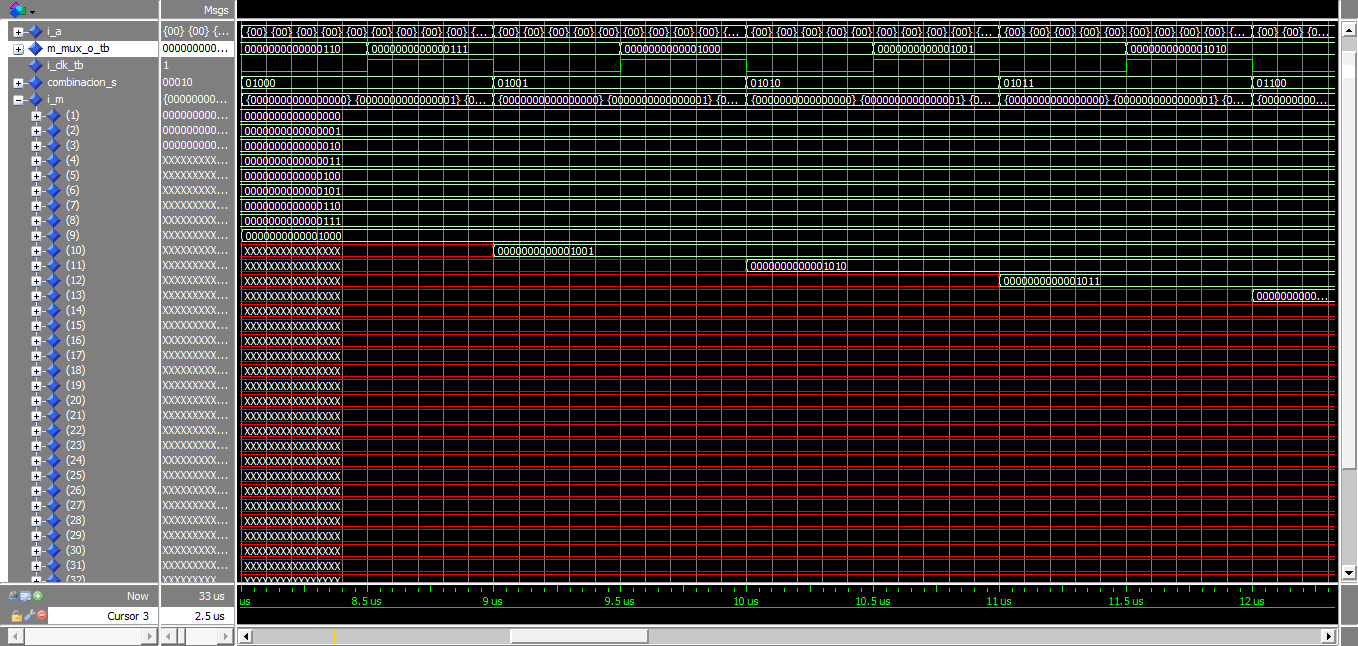
\includegraphics[scale=0.5, angle=270]{./Figures/sectorizador_ensayo_1_zoom_mult.png}
\caption{Sectorizador. Ensayo 1. Acercamiento alrededor de $t = 9us$.}
\label{fig:sectorizador_ensayo_1_zoom_mult}
\end{figure}


\begin{itemize}
\item
Valor bajo equivalente al piso de ruido durante todo el periodo, excepto durante un pequeño intervalo de tiempo en la que adquiere un valor mayor. Se eligió como valor bajo \texttt{10000000000000} debido a que el conversor de alta velocidad es de 14-bit signado y el valor mencionado corresponde al cero. Físicamente el piso de ruido era cercano a cero. El valor de amplitud del pulso de video se eligió \texttt{10111011100000} como valor cercano al $50\%$ del rango de operación.


\item
Periódica de periodo suficientemente largo para que exista un solo pulso en el intervalo de tiempo que comprende la totalidad de celdas CFAR. La totalidad de las celdas CFAR generan un retardo indicado en la ecuación \ref{Eq:delay_cfar}, donde $N_{rc}$ es igual al número total de las celdas de referencia (128), $N_{gc}$ es igual al número total de las celdas de guarda (10) y $N_t$ es igual a el número total de las celdas bajo testeo (1).

\end{itemize}






\subsubsection{Configurador. Ensayo 2}
\label{Subsec:Configurador. Ensayo 2}
Se simuló el \textit{test bench} del componente \textit{ajuste de multiplicador}, instancia del Configurador. El intervalo de simulación estuvo entre $0 us$ y $22 us$. Se introdujo las siguientes señales de estímulo:

\begin{itemize}

\item
\texttt{i\_decision\_tb}: Señal de decisión, con valor inicial \texttt{01}, \texttt{10} luego de $3 us$, \texttt{00} luego de $13 us$ y \texttt{01} luego de $19 us$.

\item
\texttt{i\_sub\_mode\_tb}: Configuración de submodo, con valor inicial \texttt{0} y \texttt{1} luego de $2.5 us$.

\item
\texttt{i\_clk\_tb}: Señal de reloj, de periodo igual a $1 us$.

\item
\texttt{i\_rst\_tb}: Señal de reset, con valor constante $0$.

\item
\texttt{i\_multiplier\_tb}: Señal de multiplicador, con valor constante \texttt{11110000000000} ($15360$ en sistema decimal).

\end{itemize}

\begin{figure}
\centering
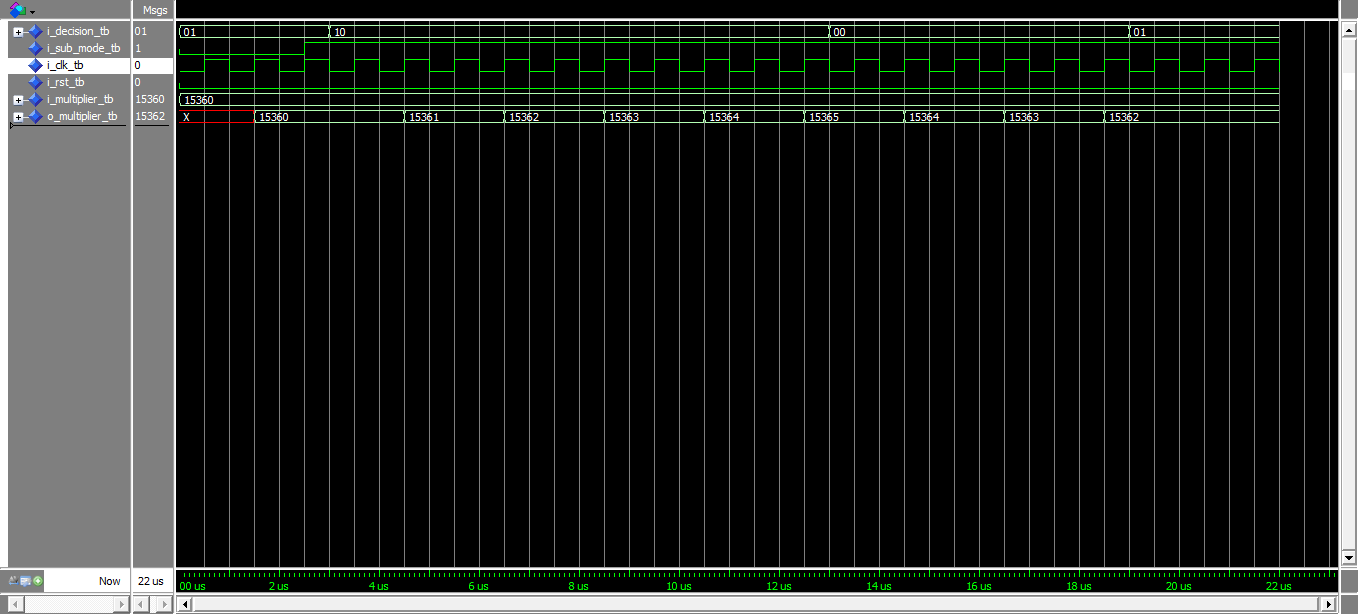
\includegraphics[scale=0.52, angle=270]{./Figures/multiplier_setting_ensayo_1.png}
\caption{Configurador. Ensayo 2}
\label{fig:multiplier_setting_ensayo_1}
\end{figure}

El resultado se ilustra en la figura \ref{fig:multiplier_setting_ensayo_1}. Un valor de decisión \texttt{01} significa "no realizar modificaciones al multiplicador", en otras palabras: dejar ese valor constante. Un valor de decisión \texttt{10} significa ''incrementar el valor del multiplicador en un delta''. Donde el \textit{delta} tuvo valor $1$ por defecto. Por último, un valor de decisión \texttt{00} significa ''decrementar el valor del multiplicador en un delta''. La señal del multiplicador de entrada es constante debido a que el mismo se almacena en un registro externo al módulo e interno a cada sector, se toma dicho valor como referencia.

Se observó que para $t = 1.5 us$, luego de $2$ flancos ascendentes de reloj, la salida queda definida en el valor configurado desde la entrada. Este valor se mantiene constante entre $t = 1.5 us$ y $t = 3 us$, intervalo de tiempo en el que el submodo estuvo con valor $0$ correspondiente a una operación fija. A partir de $t = 3 us$ el submodo adquirió valor $1$ indicando una operación automática, esto significa que se habilita con una modificación automática del último valor del multiplicador almacenado en el registro interno al módulo en función del valor de decisión de entrada. Se observó que entre $t = 3 us$ y $t = 13 us$, intervalo de tiempo en donde la decisión tomó valor $10$, el valor del multiplicador aumentó en una unidad en cada flanco ascendente de reloj. Para el intervalo de tiempo entre $t = 13 us$ y $t = 19 us$, donde la decisión tomó valor $00$, el valor del multiplicador disminuyó en una unidad en cada flanco ascendente de reloj. Finalmente, a partir de $t = 19 us$, con el valor de decisión $01$, el valor del multiplicador permaneció constante.



\subsubsection{Configurador. Ensayo 3}
\label{Subsec:Configurador. Ensayo 3}
Se simuló el \textit{test bench} del Configurador. El intervalo de simulación estuvo entre $0 us$ y $40 us$. Se introdujo las siguientes señales de estímulo:

\begin{itemize}
\item
Para el bloque fijo:
	\begin{itemize}
	\item
	\texttt{i\_multiplier\_fxs\_tb}: Señal de multiplicador, con valor constante de \texttt{1110000000000000}.
	
	\item
	\texttt{i\_algorithm\_fxs\_tb}: Señal de algoritmo, con valor constante de \texttt{00}.   
	
	\item  
	\texttt{i\_window\_sliding\_fxs\_tb}: Señal de coeficiente de ventana deslizante, con valor constante de \texttt{0000}.
	
	\item
	\texttt{i\_tolerancia\_fxs\_tb}: Señal de tolerancia, con valor constante de \texttt{00101}.    

	\end{itemize}

\item
Para un sector en particular:
	\begin{itemize}
  	\item
  	\texttt{i\_algortihm\_cfar\_tb}: Señal de algoritmo con valor \texttt{00} durante los primeros $11 us$, luego \texttt{10}.
  
  	\item
  	\texttt{i\_sub\_mode\_tb}: Señal de submodo con valor constante \texttt{0} (modo fijo).
  
  	%\item
  	%\texttt{i_presence_required_tb}. Comento porque no interesa para éste ensayo.
  
  	\item
  	\texttt{i\_multiplier\_cfar\_tb}: Señal de multiplicador, con valor \texttt{1110000000000000} durante los primeros $11 us$, luego \texttt{1111000000000001}.
  
  	\item
  	\texttt{i\_window\_sliding\_tb}: Señal de coeficiente de ventana deslizante, con valor \textit{0100} durante los primeros $11 us$, luego \texttt{1010}.
  
  	\item
  	\texttt{i\_sector\_addr\_tb}: Señal de identificación de sector, con valor \texttt{00101} durante los primeros $11 us$, luego \texttt{00011}.
	\end{itemize}

\item
Señales comunes:
	\begin{itemize}
	\item
	\texttt{i\_clk\_tb}: Señal de reloj, de periodo igual a $1 us$.
	
	\item 
	\texttt{combinacion\_s}: Señal de $5\-bit$, que incrementó su valor en cada flanco ascendente del reloj y que produjo el efecto de realizar un barrido por todos los sectores.
	
    
    \item
    \texttt{i\_mode\_tb}: Señal de modo de operación, con valor \texttt{0} (no sectorizado) durante los primeros $10 us$, luego \texttt{1} (sectorizado).
    
    \item
    \texttt{i\_load\_config\_tb}: Señal de carga de configuración a un sector determinado, consiste en un pulso de una duración de $1 us$. Se generó dos pulsos de carga de configuración, el primero a los $2 us$ y el segundo a los $13 us$.
    
    \item
    \texttt{i\_tolerancia\_tb}: Señal de modo de tolerancia, con valor constante \texttt{10} (2 en sistema decimal).
    
    \item
    \texttt{i\_passed\_through\_north\_tb}: Señal de paso por el norte, consiste en un pulso de una duración de $1 us$. Se utilizó esta señal para actualizar la salida de todos los sectores del modo sectorizado. Se generó dos pulsos de paso por el norte, el primero a los $7 us$ y el segundo a los $18 us$. Es necesario que estos pulsos se produzcan después de  el pulso de carga de configuración para que la salida presente el valor configurado con el pulso de carga mencionado.
	\end{itemize}

\end{itemize}



\begin{figure}
\centering
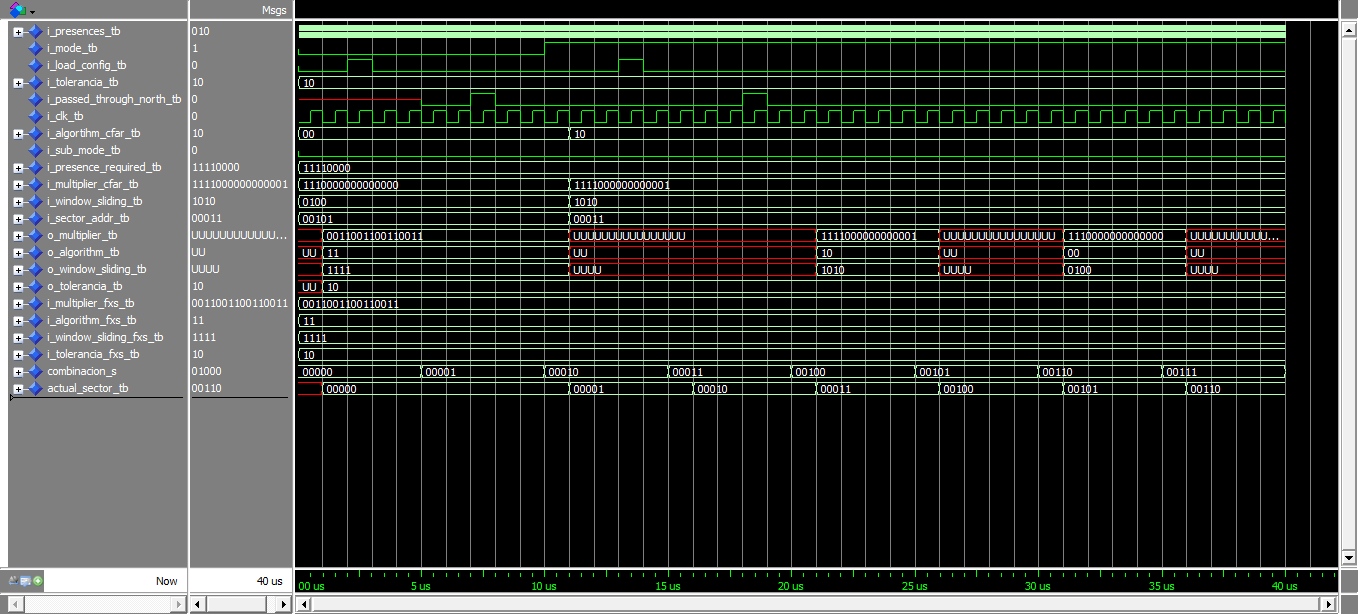
\includegraphics[scale=0.52, angle=270]{./Figures/configurador_ensayo_3.png}
\caption{Configurador. Ensayo 3}
\label{fig:configurador_ensayo_3}
\end{figure}


El resultado se ilustra en la figura \ref{fig:configurador_ensayo_3}. Se observó que durante los primeros $10 us$ la señal de modo permanece en $0$. Debido a esto la salida de los sectores con \textit{id} \texttt{00000} y \texttt{00001} son ignoradas mientras el sector actual adquiere estos valores, en cambio la salida del configurador adopta los valores de multiplicador, algoritmo, coeficiente de ventana y tolerancia del sector fijo. Esta salida tiene lugar desde el tiempo $t = 1 us$ en el flanco descendente del reloj, estando indefinida por este motivo en el momento inicial. Cabe mencionar que para asegurar la estabilidad de los datos al momento de la lectura por parte del CFAR, se eligió para la salida del configurador como flanco activo el flanco descendente. De esta manera se produce un desfase entre la actualización del dato a la salida de este módulo y la lectura del dato a la entrada del CFAR.

Luego de los $10 us$ se observó que la señal de modo conmutó a $1$. Esto produce un cambio en la salida del configurador. En modo sectorizado se ignora la salida del sector fijo y se considera la salida de los $32$ sectores restantes, proporcionando a la salida del configurador la configuración almacenada para el sector correspondiente al sector actual. Debido a que se configuró sólo dos sectores, se observó que la salida del configurador estuvo indefinida para aquellos sectores que no fueran los que se configuraron.

En $t = 21 us$, cuando el sector actual cambia de valor de \texttt{00010} y \texttt{00011}, las salidas del configurador adpotan los valores configurados para el sector \texttt{00011} de acuerdo a los estímulos generados. Una situación similar ocurre para $t = 21 us$ con el sector \texttt{00101}



\subsection{Resultados a ensayos con visores de netlist}
\label{Subsec: Resultados de Visores de netlist}

\begin{figure}
\centering
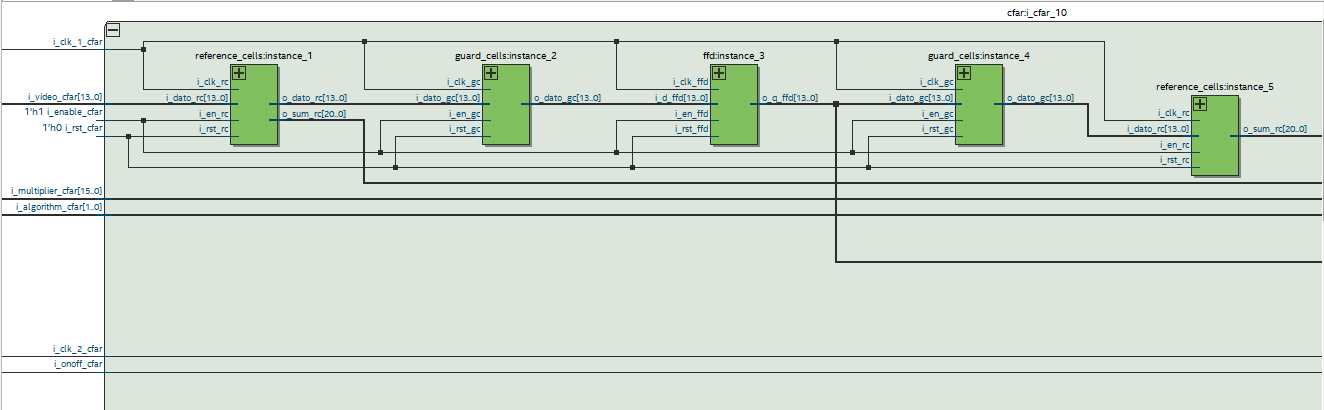
\includegraphics[scale=0.6, angle=270]{./Figures/RTL_cfar_1.png}
\caption{Diagrama RTL de la sección de entrada del módulo CFAR}
\label{fig:RTL_cfar_1}
\end{figure}


\begin{figure}
\centering
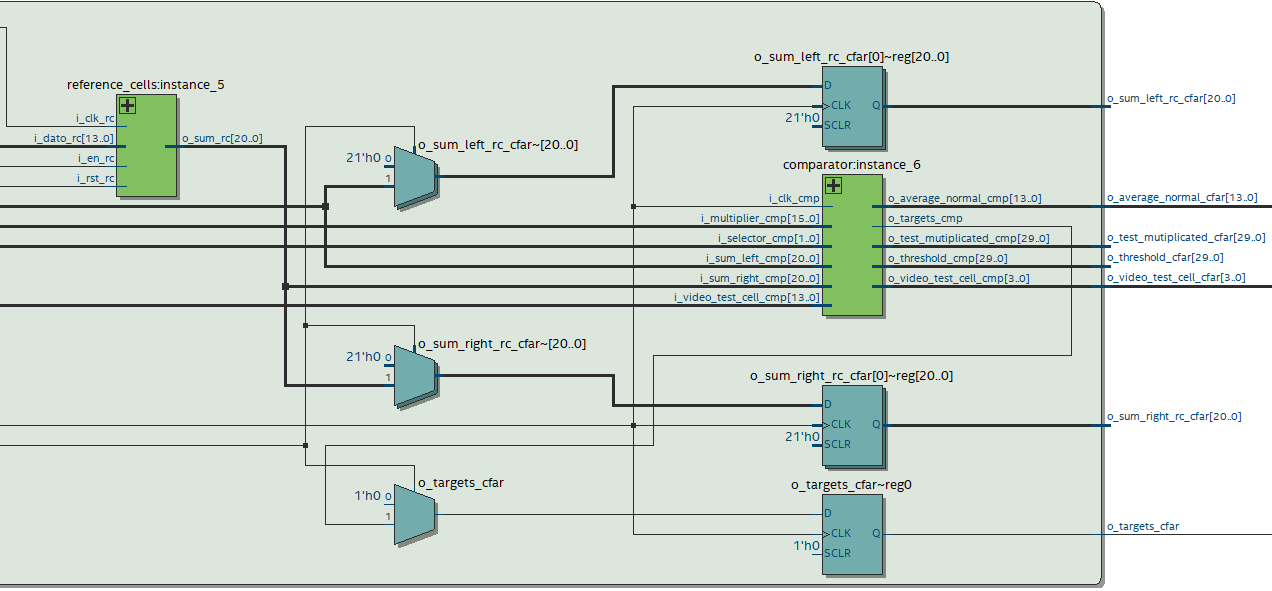
\includegraphics[scale=0.5]{./Figures/RTL_cfar_2.png}
\caption{Diagrama RTL de la sección de salida del módulo CFAR}
\label{fig:RTL_cfar_2}
\end{figure}



\begin{figure}
\centering
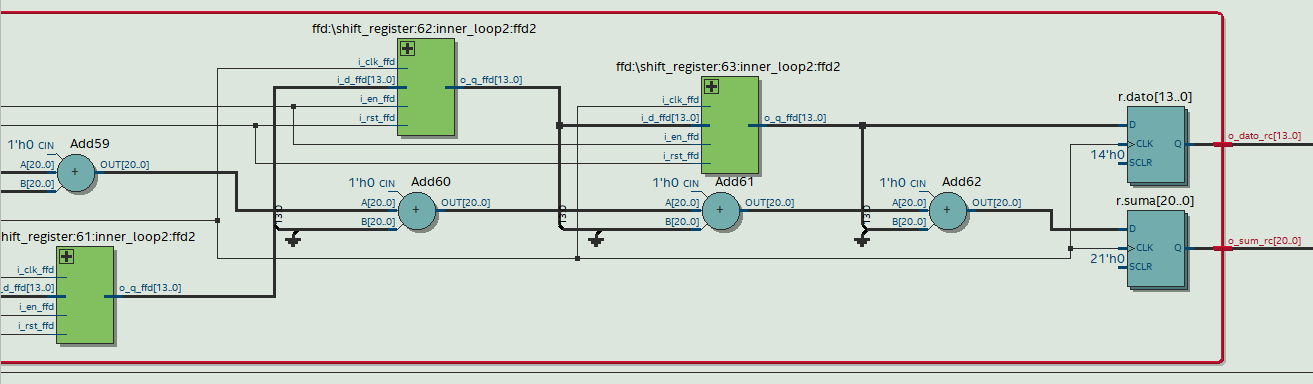
\includegraphics[scale=0.6, angle=270]{./Figures/RTL_cfar_rc_1.png}
\caption{Diagrama RTL de la sección de salida de una celda de referencia}
\label{fig:RTL_cfar_rc_1}
\end{figure}



\begin{figure}
\centering
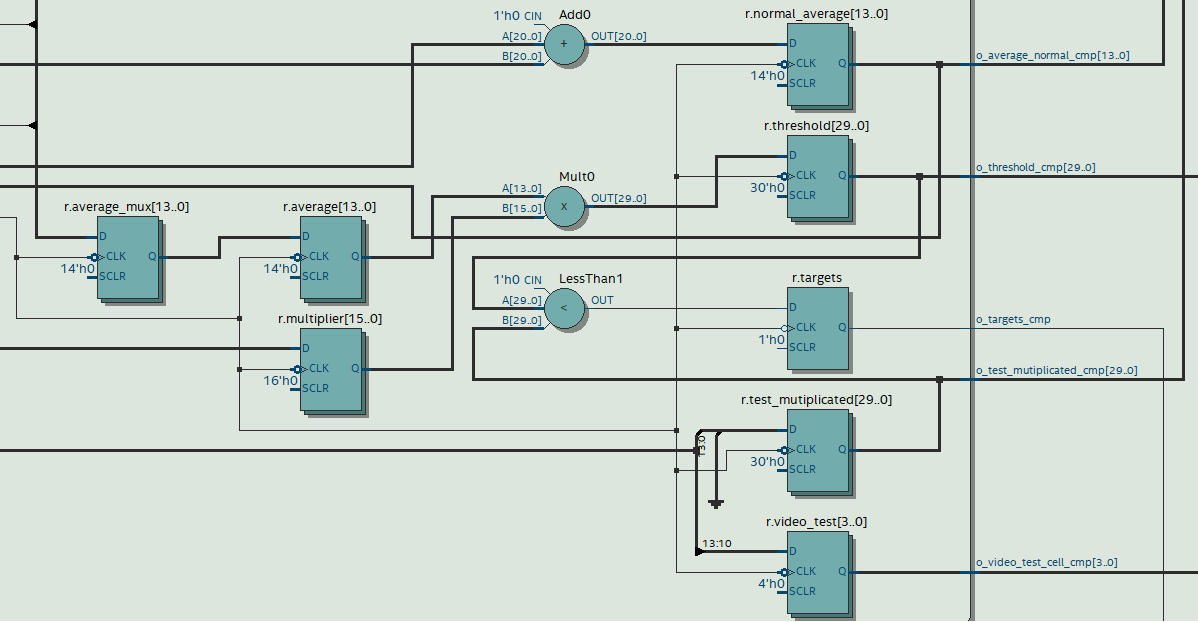
\includegraphics[scale=0.6, angle=270]{./Figures/RTL_cfar_comparador_1.png}
\caption{Diagrama RTL de la sección de salida del comparador}
\label{fig:RTL_cfar_comparador_1}
\end{figure}






\begin{figure}
\centering
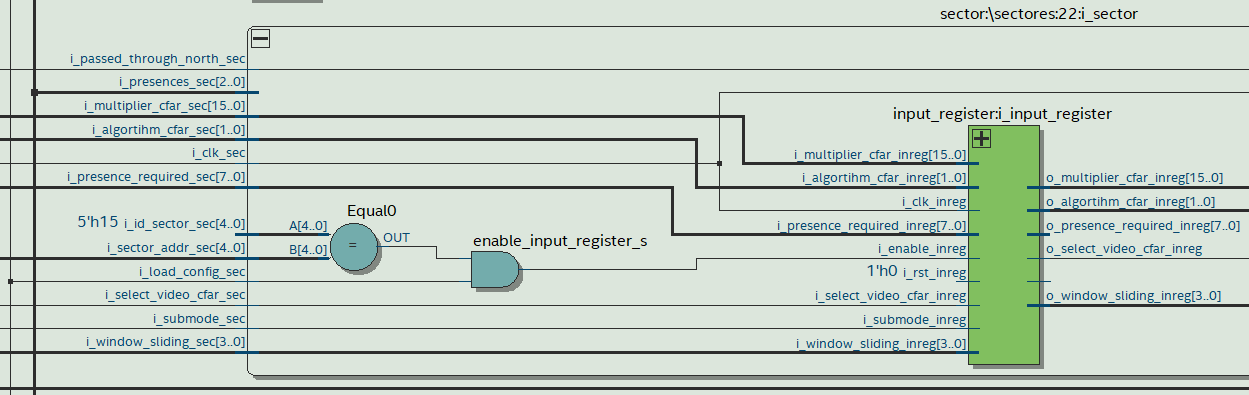
\includegraphics[scale=0.65, angle=270 ]{./Figures/RTL_cfg_sector_1.png}
\caption{Diagrama RTL de la sección de entrada de un sector}
\label{fig:RTL_cfg_sector_1}
\end{figure}



\begin{figure}
\centering
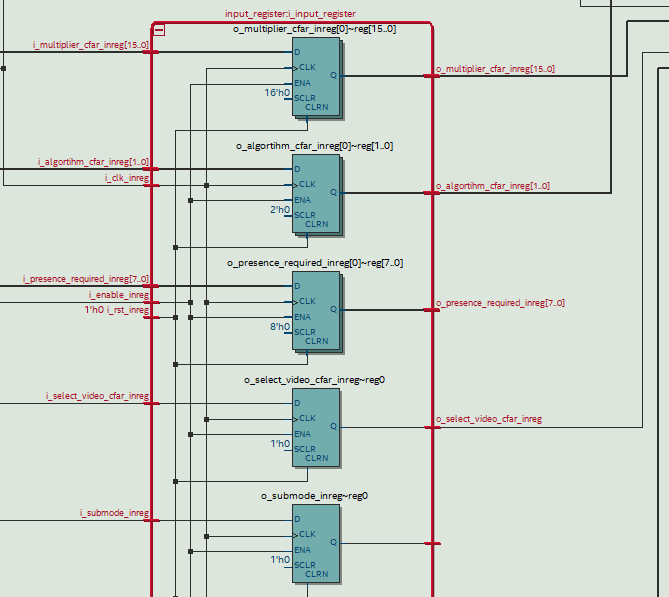
\includegraphics[scale=0.75]{./Figures/RTL_cfg_input_reg_1.png}
\caption{Diagrama RTL de una sección del registro de entrada interno a un sector}
\label{fig:RTL_cfg_input_reg_1}
\end{figure}




Se compiló el diseño del Procesador Monoradar, el cual incluyó como subsistemas a los módulos CFAR y Configurador. Superada la etapa de análisis y síntesis, fue posible utilizar la herramienta \textit{RTL Viewer} para verificar la interpretación de la herramienta de síntesis, del código RTL compilado.

Se observó el esquema RTL de las celdas CFAR, el cual se ilustra en la figura \ref{fig:RTL_cfar_1}. Los registros de desplazamientos se conectaron adecuadamente. Se verificó que todos fueron conectados a la misma fuente de reloj y compartieron las señales de habilitación y reset. Estas características permiten, según el fabricante, una adecuada inferencia de los registros de desplazamiento como tales y por tanto permiten que se efectúen procesos de optimización sobre el diseño. Se verificó además que exista una conexión serie entre estos registros. En cuanto a la sección de salida del CFAR, se verificó las conexiones del comparador y la interpretación, por parte de la herramienta de síntesis, de la lógica combinacional y secuencial de salida. Se ilustra en la figura \ref{fig:RTL_cfar_2}, los registros y \textit{flip flop} inferidos por la herramienta de síntesis a la salida del módulo CFAR. La herramienta de síntesis interpretó una lógica intermedia entre las señales provenientes de las celdas CFAR o el comparador y los registros de salida, para las señales de targets y de suma. Esta lógica consistió en una compuerta \texttt{AND} esquematizada con un multiplexor.

Desplegando uno de los módulos correspondientes a las celdas de referencia, se observó la estructura interna de esos módulos. La sección de salida se ilustra en la figura \ref{fig:RTL_cfar_rc_1}. Se observó una conexión serie de los registros, una conexión de sumadores en cascada y dos registros de salida para almacenar la suma y el video. En particular la conexión de sumadores en cascada permitió la escalabilidad del módulo; fue posible durante el diseño generar celdas de referencia con diferente cantidad de celdas sin mayores complicaciones.

Para el componente \textit{comparador} se observó la interpretación por parte de la herramienta de síntesis de un circuito combinacional y otro secuencial, acorde a la descripción realizada en la sección \ref{metodologia_estructurada} del capítulo \ref{Chapter2} sobre la \textit{metodología estructurada}. En la figura \ref{fig:RTL_cfar_comparador_1} se ilustra la sección de salida del comparador compuesta por un circuito secuencial.

En cuanto al configurador, se verificó la interpretación de la descripción RTL del módulo. Se ilustran ejemplos de los esquemas RTL del sector y del registro de entrada interno al sector, en las figuras \ref{fig:RTL_cfg_sector_1} y \ref{fig:RTL_cfg_input_reg_1}. En la figura \ref{fig:RTL_cfg_sector_1} se ilustra la condición de igualdad que debe cumplirse entre la señal de combinación de sector y la señal de identificación de ese sector, luego con una compuerta \textit{AND} se impuso otra condición para que se habilite la carga de la configuración con una señal adicional (proveniente del puente HPS). En la figura \ref{fig:RTL_cfg_input_reg_1} se ilustra parte de los diferentes componentes que componen el módulo: por un lado \textit{flip flops} tipo D para la selección del video CFAR y el submodo, y por el otro registros para la presencia requerida, algoritmo y multiplicador.




\subsection{Resultados a ensayos con simulador y decodificador}
\label{Subsec: Resultados de simulador y decodificador}

Debido a que el módulo configurador no necesitó de señal de radar real para operar, se utilizó un decodificador y un simulador para verificar su funcionamiento luego del proceso de implementación en la FPGA, como se mencionó en la sección \ref{Ensayos_simulador_decodificador} del capítulo \ref{Chapter3}. El decodificador recibió las señales de salida del configurador correspondientes a:

\begin{itemize}
\item Señal proveniente del puerto de salida del algoritmo
\item Señal proveniente del puerto de salida del coeficiente de ventana deslizante
\item Señal proveniente del puerto de salida del multiplicador
\end{itemize}

A su vez, en el interior del decodificador se almacenó una configuración para estos parámetros más una configuración adicional para otro valor de multiplicador. La configuración almacenada fue:

\begin{itemize}
\item Algoritmo: \texttt{01}
\item Multiplicador 1: \texttt{1111111111111110} (65534 en sistema decimal)
\item Multiplicador 2: \texttt{1000000000000000} (32768 en sistema decimal)
\item Coeficiente de ventana deslizante: \texttt{0011} (3 en sistema decimal)
\end{itemize}


Luego, en caso de que alguna señal de entrada del decodificador coincidiera con el valor almacenado de ese parámetro, se debía emitir un nivel lógico alto de salida. Este \textit{bit} se utilizaba para comandar cuatro \textit{leds} indicadores incorporados a la placa ADC-SoC. De esta, manera por ejemplo, cuando la señal de salida de coeficiente de ventana sea \texttt{0011} se debía encender el led correspondiente a ese parámetro, de lo contrario debía estar apagado. Además se conectó la señal de paso por el norte a otro led adicional, para visualizar el momento en el que se completaba una vuelta de radar.

Con las configuración almacenada se ejecutó el simulador de blancos implementado en la placa ADC-SoC. La parte del simulador de interés para este ensayo fue el barrido en rango y azimut, que permitió para que el configurador realice un barrido por todos los sectores implementados. Se configuró la cobertura con los dos valores almacenados en el decodificador. Se dividió la cobertura en dos, a la mitad del intervalo total de azimut. Una mitad de la cobertura (16 sectores) se configuró con con un valor de multiplicador \texttt{1111111111111110} y la otra con valor \texttt{1000000000000000}. Luego se configuró toda la cobertura con los valores de algoritmo y coeficiente de ventana deslizante almacenados en el decodificador.

Con el simulador y el procesador monoradar en ejecución, y después de realizada la configuración, se observó el encendido y apagado de los leds. Cuando el simulador completó una vuelta de radar el led de paso por el norte produjo un centelleo (breve encedido); a partir de ese momento y durante la mitad del tiempo de cobertura se encendió el led de multiplicador 1 mientras el led de multiplicador 2 estuvo apagado. Luego desde la mitad del tiempo de cobertura hasta el final de la misma se encendió el led de multiplicador 2 mientras el led de multiplicador 1 estuvo apagado. Los leds correspondientes al algoritmo y al coeficiente de ventana deslizante estuvieron encendidos sólo durante la mitad del tiempo de cobertura debido a que sólo una mitad de la cobertura se configuró para cumplir con la condición del decodificador.

\subsection{Resultados a ensayos con procesador monoradar preexistente}
\label{Subsec: Resultados a procesador monoradar preexistente}

Se realizaron pruebas con un radar FPS113 de la Fuerza Aérea Argentina. Se utilizó un procesador monoradar preexistente para verificar el funcionamiento del CFAR luego del proceso de implementación en la FPGA, como se mencionó en la sección \ref{Ensayos_Procesador_Monoradar_preexistente} del capítulo \ref{Chapter3}. No se empleó el simulador debido a que para verificar el funcionamiento del CFAR fue necesario contar con señal de radar real.

Se utilizó un decodificador para visualizar con unos leds incorporados en la placa ADC-SoC la cuenta de targets del CFAR en una vuelta de antena. Esto se llevó a cabo con el módulo \textit{contador CFAR} el cual consistió en un acumulador que proporcionaba 4 salidas de 1-bit correspondiente a los 4 bits más significativos de la cuenta. Se verificó que para en cada vuelta de antena se obtiene una cuenta ascendente de targets que se reseteaba en la vuelta de antena siguiente.

Se empleó el procesador monoradar preexistente para realizar una comparación con el nuevo procesador monoradar del cual los subsistemas diseñados en este trabajo fueron parte. Se verificó que los blancos detectados por ambos sistemas coincidían en valores de rango y azimut, lo que significó que para la misma señal de entrada se produjo resultados similares. 
% Chapter Template

\chapter{Conclusiones} % Main chapter title

\label{Chapter5} % Change X to a consecutive number; for referencing this chapter elsewhere, use \ref{ChapterX}


%----------------------------------------------------------------------------------------

%----------------------------------------------------------------------------------------
%	SECTION 1
%----------------------------------------------------------------------------------------

\section{Conclusiones generales }

La idea de esta sección es resaltar cuáles son los principales aportes del trabajo realizado y cómo se podría continuar. Debe ser especialmente breve y concisa. Es buena idea usar un listado para enumerar los logros obtenidos.

%----------------------------------------------------------------------------------------
%	SECTION 2
%----------------------------------------------------------------------------------------
\section{Próximos pasos}

Acá se indica cómo se podría continuar el trabajo más adelante.
 

%----------------------------------------------------------------------------------------
%	CONTENIDO DE LA MEMORIA  - APÉNDICES
%----------------------------------------------------------------------------------------

\appendix % indicativo para indicarle a LaTeX los siguientes "capítulos" son apéndices

% Incluir los apéndices de la memoria como archivos separadas desde la carpeta Appendices
% Descomentar las líneas a medida que se escriben los apéndices

%% Appendix A

\chapter{Appendix Title Here} % Main appendix title

\label{AppendixA} % For referencing this appendix elsewhere, use \ref{AppendixA}

Write your Appendix content here.
%\include{Appendices/AppendixB}
%\include{Appendices/AppendixC}

%----------------------------------------------------------------------------------------
%	BIBLIOGRAPHY
%----------------------------------------------------------------------------------------

\Urlmuskip=0mu plus 1mu\relax
\raggedright
%\printbibliography[heading=bibintoc]

%----------------------------------------------------------------------------------------

\end{document}  
